\chapter{\label{ch:frag_char}Characterizing Chemical Fragmentation Definition Through Unsupervised Learning Methods}


The author's contribution to the work included development of descriptors, writing of code, running calculations, performing analysis, and writing/editing the manuscript. This work is in preparation and will be submitted shortly \textcolor{red}{I don't know what phrasing to use here.}

\section{Summary}
In order to reduce the computational cost of large calculations, we look to fragmenting large molecules into smaller subsystems which can best represent the whole.
This work proposes a scheme for automatic molecular fragmentation through unsupervised learning approaches in which each fragment is chosen to best retain the important features of the bonding environment.
This chapter highlights the efforts at benchmarking the performance of our proposed method on a set of test systems.
%what as done
To this end, a set of clustering algorithms (spectral, agglomerative, $k$-means, and affinity propagation) were studied in combination with various molecular representations, including those incorporating bonding information derived from quantum mechanics.
The performance for the clustering/descriptor combinations was assessed for test systems spanning a range from easily distinguishable fragments such as non-covalently bound water cluster to oligomers in which lowest-loss fragmentation is ambiguous.
% the following needs to be updated:
Overall, it is found that spectral clustering works well in all systems tested, showing very little sensitivity to the representation employed.
Spectral, agglomerative, and $k$-means clustering produce reasonable fragments for systems with clear fragmentation patterns. Though in the oligomer system, spectral clustering achieves the best performance as assessed by offering a trade-off between lowest error and highest speed-up and is thus recommended as the most robust clustering approach for molecular systems.
% A clustering algorithm which chooses the number of clusters based on the data worked well for the water clusters, though better representations are needed for this to be used on larger systems.
The approach has the potential to improve reproducibility and transferability by replacing manual fragmentation with quantitative partitioning criteria.
\section{Introduction}
 Common quantum chemistry methods that provide an accurate description of molecules are often restricted to small systems in terms of number of atoms or basis set size due to high scaling of the computational cost with system size, $N$. 
% Many the accurate description of important chemical processes can rely on methods which accurately capture electron correlation.
% Although, these beyond mean-field methods are associated with higher scaling.
For example, coupled-cluster singles doubles with perturbative triples methods is often regarded as the``gold standard" level of theory, but incurs an $N^7$ scaling. Full configuration interaction (FCI), which is formally exact in a complete basis, has prohibitive $N!$ scaling.
The higher scaling restricts the application of these methods to small systems while many of the chemical processes of interest involve large molecules.
% However, the correlation energy is known in many systems to be a very localized behavior. 
To compensate for this high scaling, fragmentation approaches estimate the energy and other properties of large molecular systems by partitioning the system into small subsystems, where the final estimate of the energy becomes the accumulation of the parts.
The accuracy of this approach hinges on the electronic structure treatment of each fragment, the approach used to describe the interaction between the fragments, and the way in which the molecule is partitioned.
The possible inter- and intra-fragment treatment approaches are vast, but beyond the scope of the current article, though interested readers are directed towards a number of helpful reviews.\autocite{Herbert2019,gordon_fragmentation_2012}
In the fragmentation schemes, the best case scenario for scaling becomes $\mathcal{O}(N^p)\ \rightarrow N_{\textrm{frag}} \mathcal{O}(f^p)$,
where $N_{frag}$ is the number of fragments, $f$ is representative of the fragment size, and $p$ is the exponential value dependent on the level of electronic structure theory utilized.\autocite{Herbert2019,hasegawa_fragment-based_2013}
This partitioning of a single, very costly calculation into $N_{frag}$ smaller calculations achieves two important objectives:
1) Computational scaling with system size is reduced with reasonable fragment definition and
2) trivial parallelization is possible by treating subsystems separately, with the potential to efficiently utilize high performance computing resources. 
In addition to enabling the treatment of larger systems, fragmentation methods can provide detailed insight into interfragment interactions when combined with analysis techniques such as energy decomposition analysis or symmetry adapted perturbation theory.\autocite{jeziorski_perturbation_1994,sapt1,Lambrecht2019,Berquist2018,Khaliullin2007}
Fragmentation approaches can also assist recent efforts of enabling quantum chemistry via quantum computers. 
Current quantum computation is restricted as the integrity of the results can be sacrificed due to interactions of the hardware with the environment. Fragmentation methods have been suggested as ways to treat larger molecular systems on quantum computers.
By breaking molecules into smaller domains before treatment on a quantum computer, the most important chemical interactions can be efficiently described without succumbing to errors resulting from the quantum computing hardware.\autocite{yamazaki2018practical}

As pointed out by Herbert, the choice of fragments for a system is not well-defined, but affects the quality of results obtained.\autocite{Herbert2019}
In some systems, a natural approach towards partitioning arises when there is a stark difference in the types of bonding present in the system, such as in non-covalent molecular clusters. 
For covalent systems, however, the choice of fragments is not always as clear-cut. 
In such cases, fragmentation requires the comparison of total energies, dipoles, or polarizabilities.
Often the fragment definition is based on predefined functional groups or chosen manually.\autocite{muller_flexible_2019}
Some methods of energy estimation are defined based on specific fragmentation schemes such as the systematic molecular fragmentation (SMF) and systematic molecular fragmentation by annihilation (SMFA).\autocite{doi:10.1063/1.1879792,10.1063/1.2347710,10.1063/1.3222639,C2CP23832B,Kobayashi2019}
In these methods, fragments are built around functional groups or larger fragments made from their groupings.
Ultimately, the level of fragmentation is at the discretion of the user to achieve the desired level of accuracy.
However, functional group definition may become ambiguous.
For example, there is no set number of monomers to include from a polymer backbone to acquire and accurate description capture the chemical behavior.
Additionally, a fragment definition based only on functional groups may not consider the interacting chemical environment. 

A desirable approach to choosing fragments would have low computational cost and prioritize keeping associated molecular components intact to treat fully with quantum mechanics while the estimation of their interactions should occur only at the most weakly bound points. 
\textit{To this end, we propose an approach utilizing clustering methods to identify the strongly interacting substructures of the system, which we term Automatic Fragmentation of Molecules using Clustering (AFMC) approach.}
Clustering methods are a form of unsupervised machine learning used to identify substructures in data sets, as a result these approaches are fundamental to data-mining procedures.
Previous work in chemistry utilized clustering methods to identify structure-property relationships in large databases\autocite{Huan2016}, to determine the number of residues to treat in quantum refinement methods\autocite{zheng_solving_2017}, and to partition large proteins into peptides using an amino acids representation using graph based methods.\autocite{10.1021/acs.jctc.0c01054}
The application of clustering methods to produce logical fragments of individual molecules at an atomic level is an unexplored direction.
The motivation is that these unsupervised machine learning algorithms (UML) , given a certain level of molecular information, will be able to group the atoms interacting most strongly with each other, ensuring that segmentation occurs between atoms which are the most weakly connected. 
This approach is able to operate independent from functional group definition which will become useful for capturing non-covalent interactions and non-local interactions in materials or biomolecules.
Additionally, this approach is expected to overcome shortcomings in other fragmentation approaches such as severing of double bonds or ring structures, since the molecular representation should be designed to avoid this.

The article is organized as follows, Section~\ref{sec:frag_approach} will discuss the clustering approaches used, Section~\ref{sec:frag_desc} will describe the representation of chemical data used as input for the clustering approach, with validation methods described in Section~\ref{sec:frag_val}, results and a discussion on clustering performance follow in Section~\ref{sec:frag_results}. 
\section{Methods}
In UML approaches, the clustering depends fundamentally on two factors: the features used to describe each data point and the algorithm used to identify domains within the data. 
This section introduces UML (clustering) approaches along with molecular representations (features) upon which fragment selection is based. 
Additionally, metrics are discussed to assess the quality of a chosen partitioning and molecular test systems are presented.
%The features of each data point are referred to as the representation. 
Four representations are explored in this work and are described in Section~\ref{sec:frag_desc}.
Several clustering approaches selected from a range of different families of algorithm were considered. 
The main article focuses on agglomerative, $k$-means, and spectral clustering; additional algorithms tested can be found in the supporting information.
These clustering methods are described in Section~\ref{sec:frag_approach}.
The code used to explore automatic molecular fragmentation using clustering can be found at \url{https://github.com/amandadumi/molfrag}. 
Clustering approaches are utilizing the implementations contained within the scikit-learn Python package.\autocite{scikit-learn}



\subsection{\label{sec:frag_approach} Clustering approaches}

This subsection describes the clustering methods explored in this work.
This work explores the application of three clustering algorithms, representing different approaches for the selection of fragments:  agglomerative, $k$-means, and spectral clustering.\autocite{10.1093/comjnl/16.1.30,10.1093/comjnl/20.4.364,1056489,zbMATH03129892,ng_spectral_2002}
% Affinity propagation attempts to automatically determine the number of clusters.\autocite{frey_clustering_2007} 
At a minimal level, all chosen algorithms require only one user input: the number of subsets to identify within the data, i.e. the desired number of fragments. 
Starting from this user input, the clustering approaches automatically determine fragments based on selected molecular representations, as outlined below.
 

Agglomerative clustering\autocite{Ward1963} is performed in a bottom-up fashion where in each iteration the most similar clusters are merged. 
In the initial iteration, all of the atoms are regarded as individual clusters, which are then merged into larger clusters. 
Merging occurs according to a linkage criterion which describes the similarity (or distance) between clusters.
In this work, the Ward linkage criterion is used, which chooses which clusters so that the variance of Euclidean distances within each cluster is minimized.
Here, the variance of a cluster is calculated as the residual sum of squares (RSS) of all variables in a cluster $C$,
\begin{equation}
d_{C} = \sum_{i,j \in C} ||x_{i} - x_{j}||^2,
\end{equation}
where $i,j$ are observations (atoms) within a cluster with associated data points $x$. 
The Ward criterion\autocite{Ward1963} results in a more regular distribution of cluster sizes compared to other choices, which is advantageous for the speed in a fragment calculation, as even distribution of fragment sizes is associated with equal computational cost distribution.
This process is repeated until the user-specified number of fragments has been obtained. 
A visualization of this algorithm is shown in Figure~\ref{fig:methods}, where the progression of this algorithm can be understood as a dendrogram.
The dots are grouped through iterations until the desired number of clusters are found.
The time complexity of the agglomerative clustering method is $\mathcal{O}(n^3)$, but can be reduced to $\mathcal{O}(n^2)$ with various optimizations, where $n$ is the number of data points.\autocite{10.1093/comjnl/16.1.30}
A shortcoming of this method is that it is a greedy algorithm, or in other words once an atom is assigned to a fragment only considering the local environment and this assignment will not be reassessed. 

\begin{figure}
    \centering
    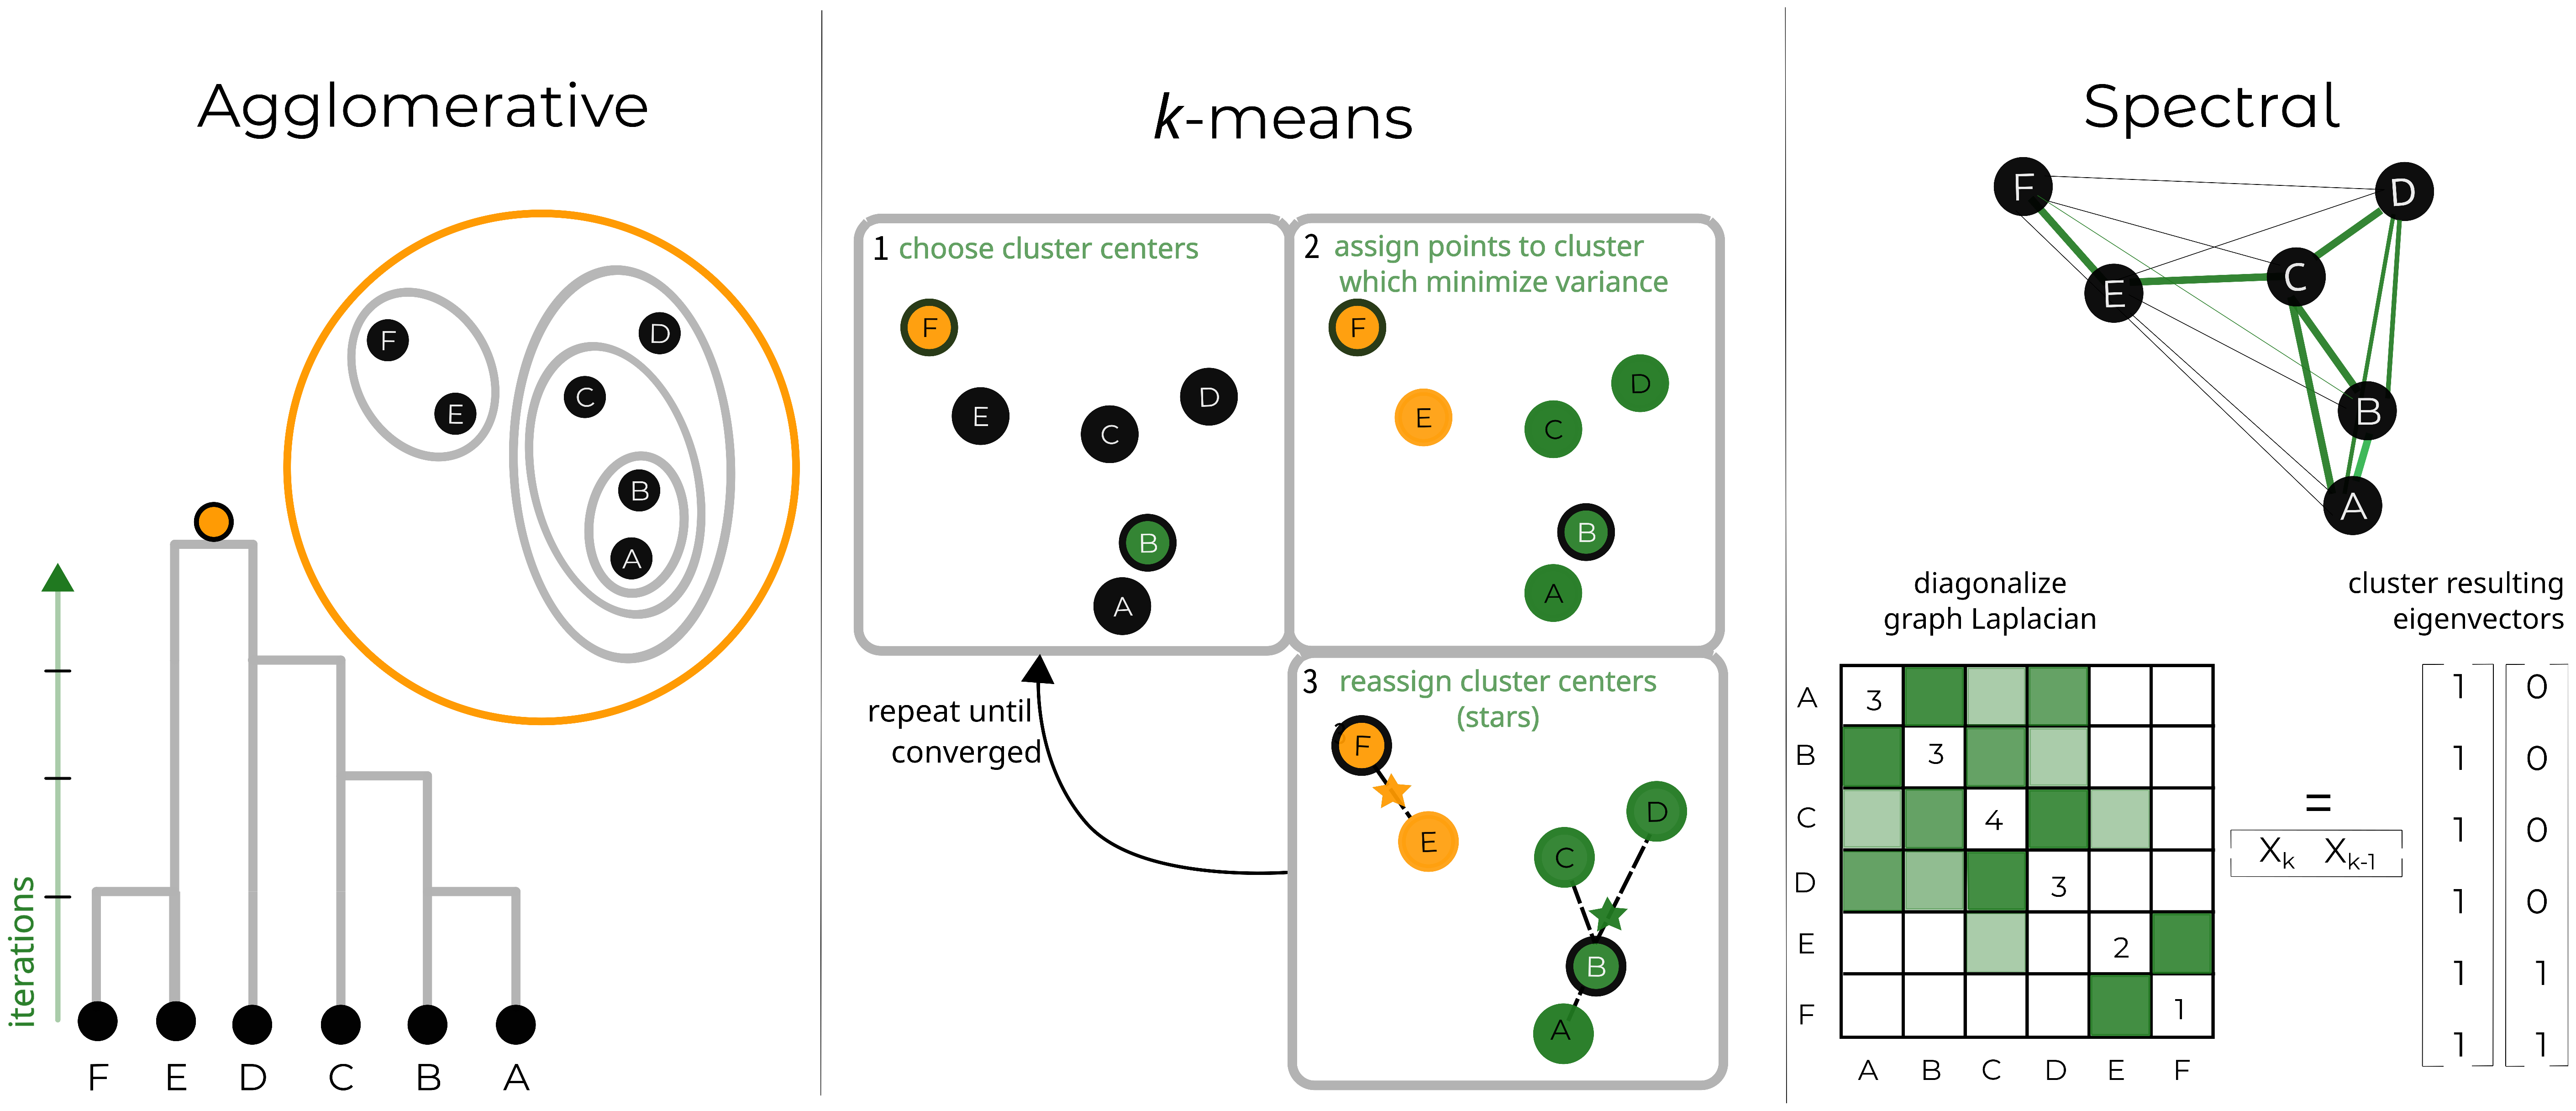
\includegraphics[width=0.9\columnwidth]{chapters/project_fragment/images/methods.eps}
    \caption[Visual representations of the clustering approaches explored]{Visual representations of the three clustering approach explored in this work. The dots are a minimal example of a set of data.
    Agglomerative clustering (left), $k$-means clustering (center), and spectral clustering (right). Detailed descriptions of each method are found in the text.}
    \label{fig:methods}
\end{figure}
The $k$-means clustering approach which iteratively minimizes the distance between the data points $x_{i}$ and the cluster centers $\bar{x}_{c}$ according to: 
\begin{equation}\label{eq:km}
\text {Minimize } \left\{ J \equiv \sum_{c=1}^{k} \sum_{i=1}^{n_{c}}\left\|x_{i}^{(c)}  - \bar{x}_{c}\right\|^{2}\right\}
\end{equation}
where $c$ denotes a particular cluster, $x_i^{(c)}$ a data point within this cluster, and $\bar{x}_{c}$ is the centroid associated with cluster $c$. 
$k$ is the number of fragments requested by the user. 
During the first iteration, the centroids are chosen randomly among the data points. 
Data points are then assigned to different centroids (clusters) based on shortest distances; centroids are updated by averaging over the data points associated with a given cluster,
\begin{equation}
\bar{x}_{c} = \sum_{j \in c} \; x_{j}^{(c)}.
\end{equation}This procedure of assigning points based on proximity to the centroids and update of centroids is repeated iteratively until changes between centroids falls below a threshold.
An illustration of this approach is given in Figure~\ref{fig:methods}. 

It is interesting to note some differences and similarities between agglomerative and $k$-means clustering.
First, it is noted that at first glance the sum of squares used as objective function within $k$-means clustering is related to Ward's linkage criteria used within agglomerative clustering. 
However, an important difference is that the $k$-means approach is non-greedy, meaning that a reassignment of points between different clusters is possible between different iterations. 
% Unlike agglomerative clustering, the $k$-means cluster assumes no structure of the data and the cluster assignment of a point can be reconsidered as new centroids are chosen.
This property implies that $k$-means has the potential to generate a global solution, whereas agglomerative clustering aims at a locally optimal solution.
Another interesting difference is that $k$-means clustering is an iterative procedure, meaning that termination and thus runtime depend on the specific data, whereas agglomerative clustering is guaranteed to terminate after a certain number of steps when the user-requested number of clusters has been identified. 
The convergence of $k$-means clustering implementations, specifically of Lloyd's algorithm \autocite{1056489}, varies significantly between average-case and worst-case scenarios.
For typical applications, $k$-means is observed to converge in few iterations, leading to an average-case observed complexity that is linear, $O(n)$, where we use $O$ to denote an approximate, observed scaling. 
In practice, $k$-means is therefore found to be more readily applicable to larger data sets compared to agglomerative clustering.
However, we do note that under worst-case scenarios the number of iterations required for $k$-means convergence scales in a superpolynomial fashion, leading to lower bounds of $2^{\Omega(\sqrt{n})}$ for the worst-case computational scaling, where $\Omega$ denotes a lower bound.\autocite{10.1145/1137856.1137880}
%The time complexity of the $k$-means clustering method is $\mathcal{O}(n^2)$, where $n$ is the number of data points.
% The steps of the algorithm and a simplified linear visualization is presented in \autoref{fig:kmeans}.
Lastly, we note that the $k$-means procedure is typically repeated for different (random) choices of initial centroids to ensure convergence to a global minimum, since initial centroids may impact the convergence to a specific solution.
For this reason, this work reports $k$-means results over ten runs with different initial centroids for each calculation.
In contrast, agglomerative clustering always produces the same results for a given set of input data except in the case of identical cluster distances; in such a case the final clusters would depend on the sorting of the input data.\autocite{yin_implementation-induced_2020}
For molecular representations using floating point numbers to map molecular structure, it is unlikely to encounter exact degeneracies. 
However, some of the molecular representations rounding these representations to integers, it would be possible to encounter degeneracies and thus a dependency of agglomerative clustering results on sorting of the input data. 


The third clustering algorithm explored here is spectral clustering.\autocite{1238361,868688,10.1093/imaiai/iay008} 
A visualization of this method can be seen in Figure~\ref{fig:methods}.
Spectral clustering begins by defining an affinity matrix $A_{ij}$ which describes the similarity of each pair of data points,  $ij$.
In the present context, the similarity between two data points can be understood as the presence of a bond or the strength of the bond.
From the affinity matrix, a degree matrix, $D$, is built, which sums the rows of $A$ onto the diagonal of $D$. 
The off-diagonal elements of $A$ combined with and $D$ are combined to form the graph Laplacian of the data as $L$ = $D$-$A$. 
The eigenvectors and eigenvalues resulting from the diagonalization of $L$ represent the data in a lower dimension space that  leads to clearer separation for linear cuts.
Following the spectral decomposition, the eigenvalues are then clustered by another method such as $k$-means, a discretized approach, or others. \autocite{10.5555/2980539.2980649,868688,1238361}. 
In this work, the $k$-means approach is utilized.
The time complexity of the spectral clustering method is $\mathcal{O}(n^3)$, where $n$ is the number of data points.
% what is important about the algorithm
%
% In the affinity propagation clustering approach the number of clusters is chosen automatically.
% Here, we provide a breif overview, though details about the method can be found in the original manuscript by Frey et al.\autocite{frey_clustering_2007}
% By representing the data as a graph, the affinity propagation algorithm passes messages through the edges between pairs. 
% Each data point must be described by the similarity between points $s(i,k)$, which captures how well $k$ could serve as an exemplar for data point $i$.
% During each iteration, two types of cluster measurements, the responsibility and the availability, are passed between pairs of data points.
% The responsibility is a measure of how well point $k$ is a representative exemplar for point $i$.
% The availability is a measure of whether or not point $i$ should be grouped with the candidate exemplar $k$ as the this value indicates to what degree $k$ is available as a cluster center for the data point, $i$.
% The iterations cease after a certain number or until the messages passed between data points fall below a certain threshold.

Additionally, the application of affinity propagation and mean shift clustering were explored, but were unsuccessful in producing useful molecular fragments. These methods are of interest since the number of clusters are chosen automatically through an a variety of approaches to analyze the density of a given set of data. However, these methods did not produce consistent results with the molecular representations explored in this work and, in many cases, no viable subsystems resulted from the fragmentation for the representations explored in this work. Although affinity propagation had some success, it was not consistent across test sets. Results for these two additional methods are included in the SI. These finding do not rule out the possible use of these clustering methods for chemical fragmentation as a tailored the molecular representation for this method may be needed.

 \subsection{\label{sec:frag_desc}Molecular Representations}

This subsection describes the molecular representation used to describe the chemical system. 
The success of clustering depends on the representation, i.e. the features used to describe the relationship between the data points (here atoms).
This work explores the application of four different representations. Two descriptors are derived from structure information alone: Cartesian-based and a covalent radii based bond matrix-based descriptors. 
The structure-only derived representation provide a low-cost descriptor as no quantum mechanical information is incorporated.
Alternatively, incorporating bonding information from a quantum mechanical treatment should provide a more detailed descriptor, though at a higher computational cost. Two descriptors which incorporate quantum mechanic information are explored: the Mayer bond matrix descriptor and the rounded Mayer bond matrix descriptor.

The descriptors are presented in a way that they represent an affinity or similarity matrix between objects. The clustering methods utilize this information in different ways. Spectral clustering uses the affinity matrix to perform the subspace search, agglomerative clustering will invert the affinity matrix to indicate that those data points more strongly interacting are closer in space, and the $k$-mean approach will use each row of the affinity matrix as a description of the dimensions in which the vector norm is measured. 
The representation is the reciprocal of each element which is handled automatically within the \texttt{molfrag} code.

The Cartesian representation describes the position of each atom  as  $x$, $y$, and $z$ components. 
Distances between any two atoms, $A$ and $B$, are calculated via the conventional Euclidean distance, $R_{AB}\ =\ \sqrt{(x_A - x_B)^2+(y_A -y_B)^2+(z_A - z_B)^2}$.
If used as a precomputed similarity matrix to describe the strength of the interactions between molecules, the representation is given as $G^{xyz}_{AB}\ =  \frac{1}{R_{AB}}$.
In $k$-means and agglomerative clustering, the Cartesian coordinates are fed directly to the clustering algorithm. 
In the spectral clustering algorithms, the Cartesian data must be represented by an affinity matrix.
The affinity matrix, $A$, defined as describes the strength of interactions between data pairs.
% $$A_{i j}=\exp \left(\frac{-d^{2}\left(s_{i}, s_{j}\right)}{\sigma^{2}}\right)$$
% where $d$ is the Euclidean distance between $i$ and $j$ and $\sigma$ is a scaling parameter.

When a descriptor exhibits a more block diagonal structure in the descriptor, many clustering methods including those explored here are able to distinguish easily between these sections. To explore if this idea can assist in molecular fragmentation definition, a representation is constructed around a bond matrix based on the covalent radii of the atoms (cr).
The covalent radii has been used in supervised machine learning as a way to numerically capture a chemical environment, thus exploring this as a feature for unsupervised machine learning is sensible.\autocite{georgescuDatabaseFeaturesMachine2021,zhaoMachineLearningBasedPrediction2020}
This is a Boolean matrix in which one indicates the presence of a bond as determined by
$$G^{cr}_{AB}\ = \begin{cases} 1\ \text{if}\ R_{AB}\ \leq\ 1.1(A_{cr}+B_{cr})\\
 0\ \text{otherwise} \end{cases}$$
where the $G^{cr}_{AB}$ is the descriptor entry, $R_{AB}$ is the distance between atom $A$ and atom $B$, and $A_{cr}$ ($B_{cr}$) is the covalent radii of $A$ ($B$).\autocite{cordero_covalent_2008,https://doi.org/10.1002/wcms.1491}

The remaining two representations incorporate information of the bonding environment via the Mayer bond order as a surrogate for density matrix and thereby quantum mechanical bonding information.
The Mayer bond order is defined in terms of spin orbitals as:
\begin{equation}
G^{Mbm}_{A B} = 2 \sum_{\mu \in A} \sum_{\nu \in B} (\mathbf{P S})_{\mu \nu}(\mathbf{P S})_{\nu \mu},
\end{equation}
where $P$ is the density matrix and $S$ is overlap matrix in an atomic orbital basis $\mu$ and $\nu$.\autocite{10.1002/jcc} 
The Mayer bond order matrix ($G^{Mbm}$) representation is  a slight modification of the form of the values into an affinity matrix, where the magnitude of the Mayer bond matrix element represents the similarity between two atoms.
As previously mentioned, some clustering methods benefit from a more block diagonal structure of the descriptor, we also look to coarse grain the descriptor through rounding the values of the matrix. This results in the rounded Mayer bond order matrix ($G^{rMbm}$) representation which rounds $G^{Mbm}_{AB}$ according to:
\begin{equation}\label{eq:rmbm}
G^{rMbm}_{AB}\ = \begin{cases} \lceil B_{AB} \rceil, \ \text{if}\ \{B_{AB}\}\ >=0.5 \\ 
 \lfloor  B_{AB} \rfloor, \ \text{otherwise.} \end{cases}
\end{equation}
The intention of this representation is to dampen out insignificant pairs, allowing only the most strongly interacting pairs to be considered in the descriptor and making the cuts between clusters more obvious.
In general, it is expected that incorporating the bond order into the descriptor will enable the fragmentation approach to preserve bonds between the most strongly interacting parts of the molecules. 
% \begin{ruledtabular}
% \begin{tabular}{ccccc}
%     &agglomerative& k-means& spectral &affinity propagation  \\ \hline
%     Cart& \makecell{Euclidean distance\\ between points} & \makecell{unchanged } & affinity matrix &\makecell{adapted affinity matrix\\ number of bonds on diagonal}  \\
%     bm&&&&\\
%     Mbm&distance matrix & & unchanged & unchanged \\
%     rMbm&distance matrix& unchanged& affinity matrix &affinity matrix\\
% \end{tabular}
% \end{ruledtabular} 
 
 
\subsection{\label{sec:frag_val} Validation}

In this section, the means of defining successful partitioning of a molecular system is outlined.
In this work, two different approaches are used: one which ensures the expected fragmentation is produced and another that quantifies the recovered energy of the full system.
The set of water clusters and methylthiophene tetramers were chosen that should produce very clear clustering for a requested number of clusters.
The performance of the clustering methods on these test cases can be assessed through external validation, which compares the resulting cluster labels to a expected/correct cluster labels.\autocite{Hubert1985,meila_comparing_2007}
The external validation statistic used in this work is the Adjusted Rand Index (ARI).
The Rand index, \ref{eq:randidx}, measures the frequency of occurrence of agreement over the total pairs.
\begin{equation}
\label{eq:randidx}
\mathcal{R}\left(\mathcal{C}, \mathcal{C}^{\prime}\right)=\frac{N_{11}+N_{00}}{n(n-1) / 2}
\end{equation}
\noindent Here $\mathcal{C}$ is the resulting clustering and $\mathcal{C'}$ is the expected clustering consisting of $n$ total points. 
$N_{00}$ and $N_{11}$ are the number of data point pairs in the same clusters and different clusters respectively for $C$ and $C'$.
However, since there is a small probability these data points could end up in the same cluster by chance, the ARI is used.
The ARI corrects for chance by using a baseline of expected similarity from a random model.
A value close to unity represents total agreement between the expected and the actual fragmentation.
The ARI approaching zero reflects an increase in the difference between the expected and returned fragmentation. 
In the oligomer systems, the correct fragmentation is ambiguous and thus correct clustering is not known ahead of time. for these systems the percent error of the fragmented system from supermolecular energy is used as the metric of success.
%%%
% and is expressed in Equation~\ref{eq:arandidx}

% \begin{equation}
% \label{eq:arandidx}
% A R I=\frac{\sum_{i j}\left(\begin{array}{c}
% n_{i j} \\
% 2
% \end{array}\right)-\left[\sum_{i}\left(\begin{array}{c}
% a_{i} \\
% 2
% \end{array}\right) \sum_{j}\left(\begin{array}{c}
% b_{j} \\
% 2
% \end{array}\right)\right] /\left(\begin{array}{l}
% n \\
% 2
% \end{array}\right)}{\frac{1}{2}\left[\sum_{i}\left(\begin{array}{c}
% a_{i} \\
% 2
% \end{array}\right)+\sum_{j}\left(\begin{array}{c}
% b_{j} \\
% 2
% \end{array}\right)\right]-\left[\sum_{i}\left(\begin{array}{c}
% a_{i} \\
% 2
% \end{array}\right) \sum_{j}\left(\begin{array}{c}
% b_{j} \\
% 2
% \end{array}\right)\right] /\left(\begin{array}{l}
% n \\
% 2
% \end{array}\right)}
% \end{equation}
% where given a set of random clusterings $n_ij$ represents the those similar for any two clusters, $a_i$ is the number overlapping ...


\subsection{\label{sec:frag_systems} Systems}

To measure the success of the AFMC approach, families of molecules are considered to explore the performance in cases where the partitioning introducing the lowest error is apparent for noncovalently and covalently bound molecules and a case of more ambiguous fragmentation in oligomers.\\ 
\noindent\textbf{Water Clusters: } The performance of the AFMC with the various descriptors on noncovalently bound molecules, a set of water clusters were explored. 
Water clusters, \ce{(H_2O)_n} for $n$=2 to $n$=21  optimized with the TIP4P water model were used from from the Wales cluster database.\autocite{wales_cambridge_nodate, 10.1063/1.445869}

\noindent\textbf{Methylthiophenes: }To benchmark performance of the fragmentation methods on covalently bound systems with a clear desired fragmentation, a set of methylthiophene tetramers were explored. When partitioning these systems, 4 fragments were requested.
Coordinates for the tetramers were generated with Open Babel by providing a SMILES representation with defined linkage atoms, indicated by a box in Figure~\ref{fig:methylthiophene}.\autocite{OBoyle2011}
The geometry of each molecule was determined at two levels of theory to study the sensitivity of the fragmentation to small perturbations in the structure. 
The levels of theory used optimize the structures were Hartree-Fock/6-311G** and $\omega$B97X-D/6-311G**.\autocite{Chai2009, Chai2008} 
Introduction of broken bonds within the molecule were treated by hydrogen capping.
The hydrogen cap contributions were then treated by subtracting the energy of all hydrogen atoms from that of the fragment calculation. 

\begin{figure}[h!]
    \centering
    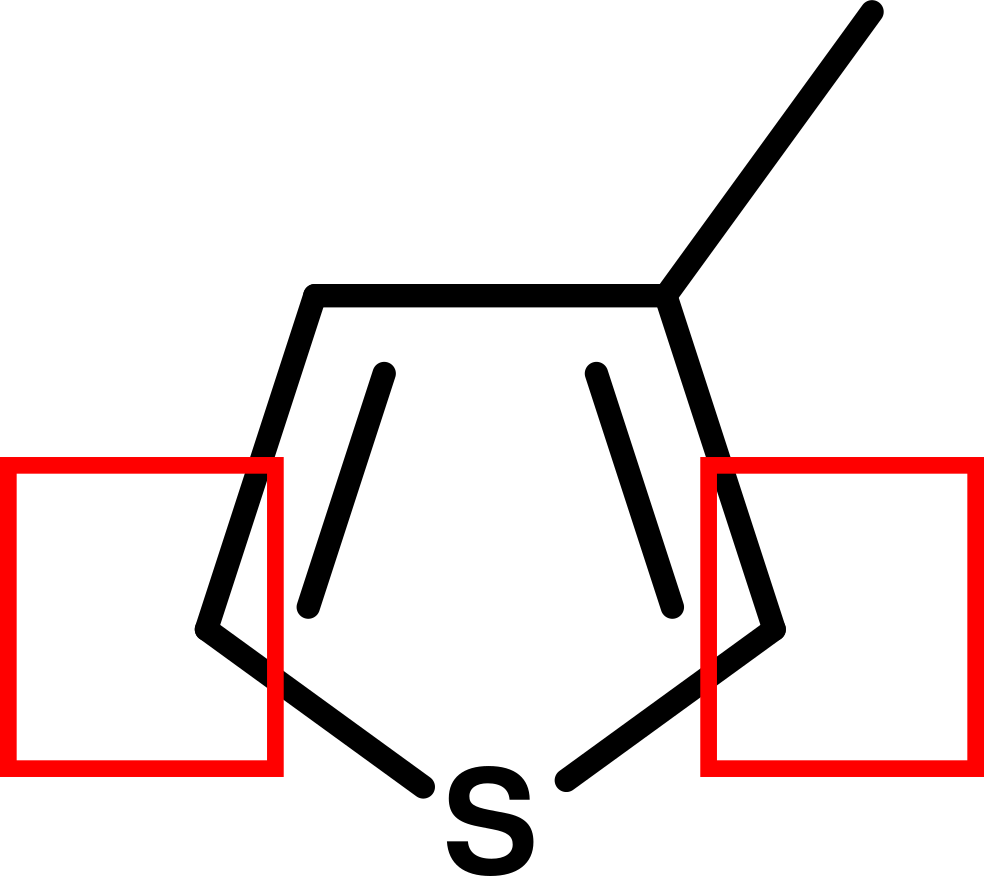
\includegraphics[width = 0.14\textwidth]{chapters/project_fragment/images/mt_monomer.png}
    \caption[The methylthiophene monomer 2-D structure]{The methylthiophene monomer 2-D structure with the linkage atoms highlighted in red.}
    \label{fig:methylthiophene}
\end{figure}

\noindent\textbf{Silyl ketene oligomers: } Silyl ketene oligomers (SKs) provide a set of systems where ideal fragmentation is ill-defined due to the backbone and side group interactions which may be essential to describe their chemistry and as a result, not clear fragmentation pattern.%, which may not be within the range of neighboring functional group definitions. 
SKs have the general form of (\ce{R}C=C=O), where R is a \ce{SiR3} group (Figure~\ref{fig:sks}(left)).
This class of molecule is a candidate for chain polymerization and can avoid the undesired 2+2 cycloadditions observed in aryl and alkyl ketenes.
Previous work in our group has aimed to predict stable structures and polymerization mechanisms.\autocite{Xiang2017}
As large polymer units are considered, the computational cost grows and fragmentation becomes an attractive and possibly necessary option.
In this work, oligomers of the SK monomers act as a test system to explore the performance of the clustering approaches in terms of the clustering ability to reduce computational time while minimize the difference in error when compared to the supermolecular calculation.
The systems explored consist of a dimer and trimer of the tert-Butyldiphenylsilyl monomer, with a methylonate nucleophile to begin the polymerization displayed in Figure~\ref{fig:sks} (center, right). 
The SK structures were generated with Avogadro2 and optimized at the Becke-3 Parameter-Lee-Yang-Parr (B3LYP) including the Becke-Johnson dispersion correction (-D3(BJ)) level of theory with the pc-1 basis set.\autocite{B3,LYP,VWN,B3LYP_assembly}
The work by Mardirossian et al. suggests this optimization level represents a balance of computational cost and accuracy. \autocite{mardirossian_thirty_2017}
Introduction of broken bonds within the molecule were treated by hydrogen capping.
The hydrogen cap contributions were then treated by subtracting the energy of all hydrogen atoms from that of the fragment calculation. 

This test case also aimed to determine the sensitivity of the clustering methods to the level of theory used for the Mayer bond order calculations.
Using the optimized structure above, the Mayer bond matrix was also calculated at varying levels of theory: Hartree-Fock, B3LYP\autocite{B3,LYP,VWN, B3LYP_assembly}, and $\omega$B97M-V\autocite{mardirossian__2016} each level of theory is paired with four different basis sets: STO-3G\autocite{hehre1969a,hehre1970a}, 3-21G\autocite{lendening1995a,andzelm1984a}, cc-pVDZ, cc-pVTZ.\autocite{ccpva,ccpvb}

\begin{figure}[h!]
    \centering
    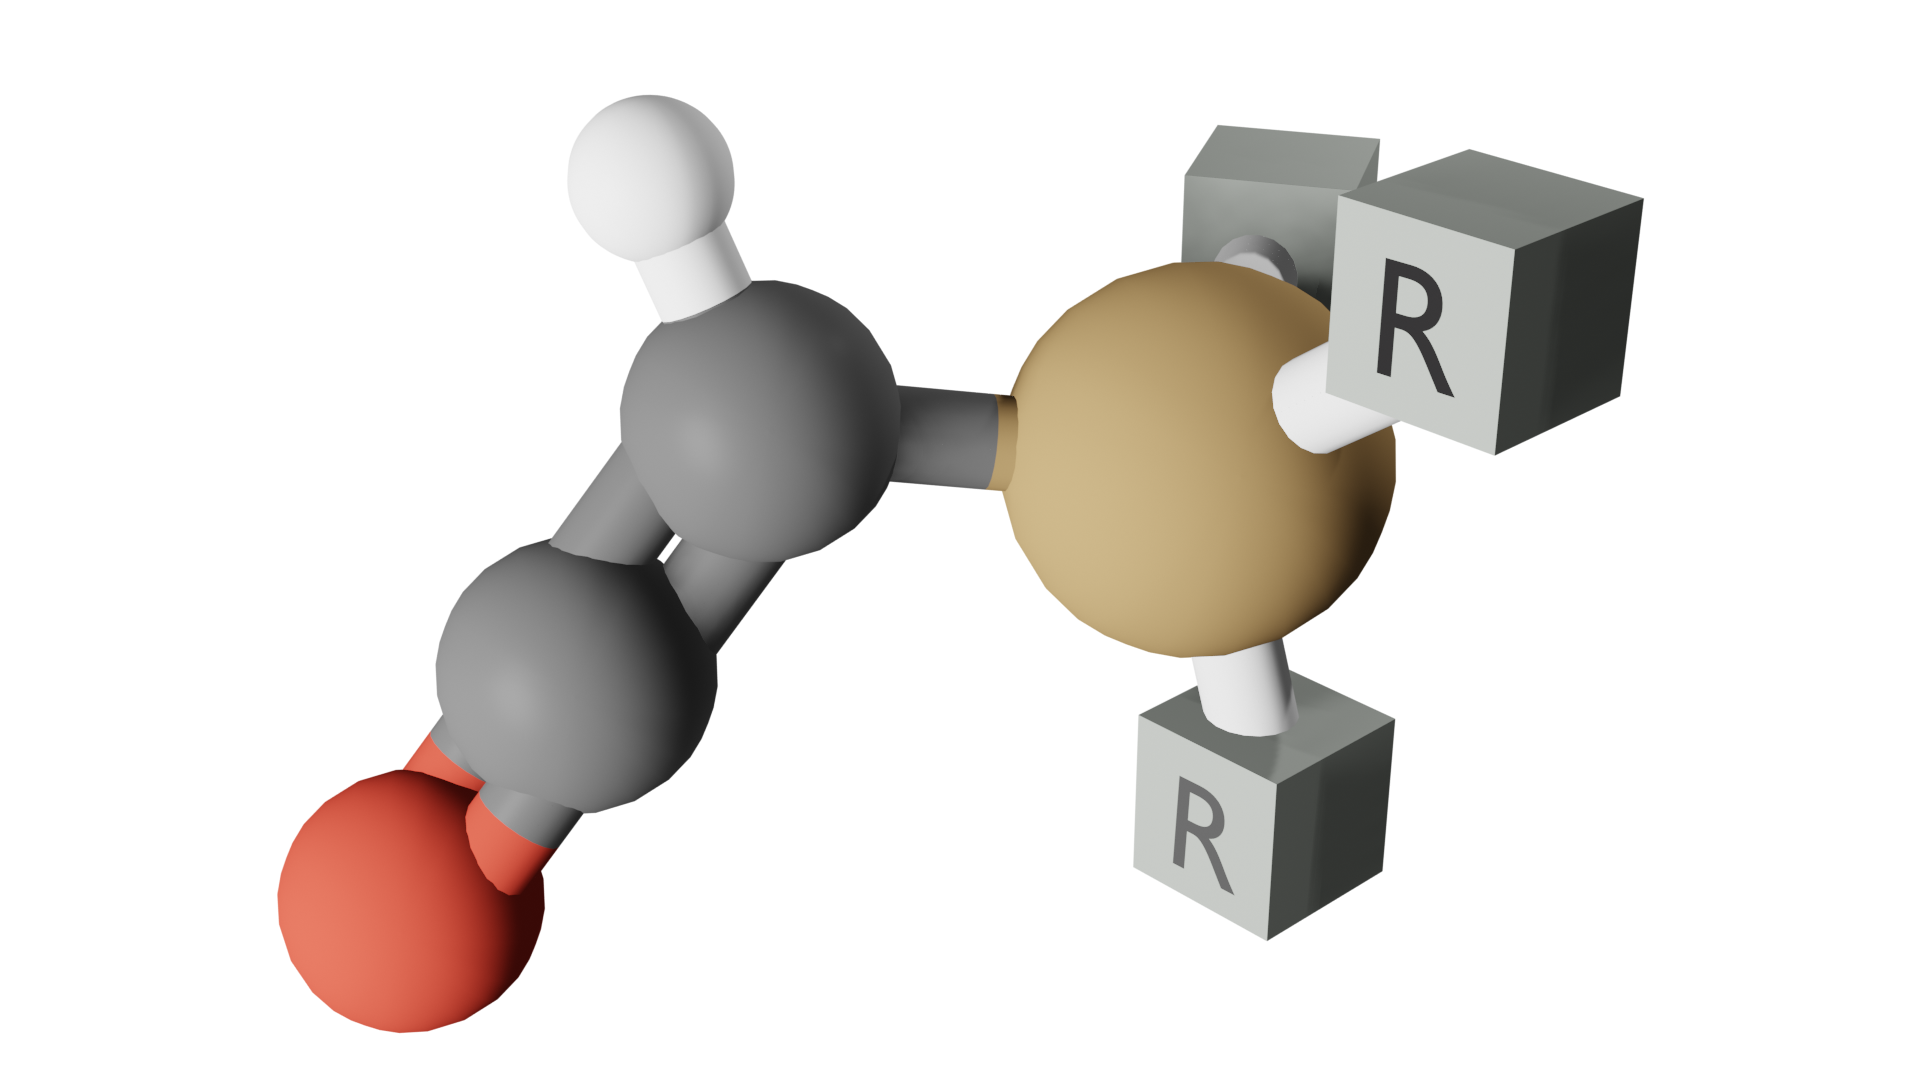
\includegraphics[width=0.3\textwidth]{chapters/project_fragment/images/base.png}     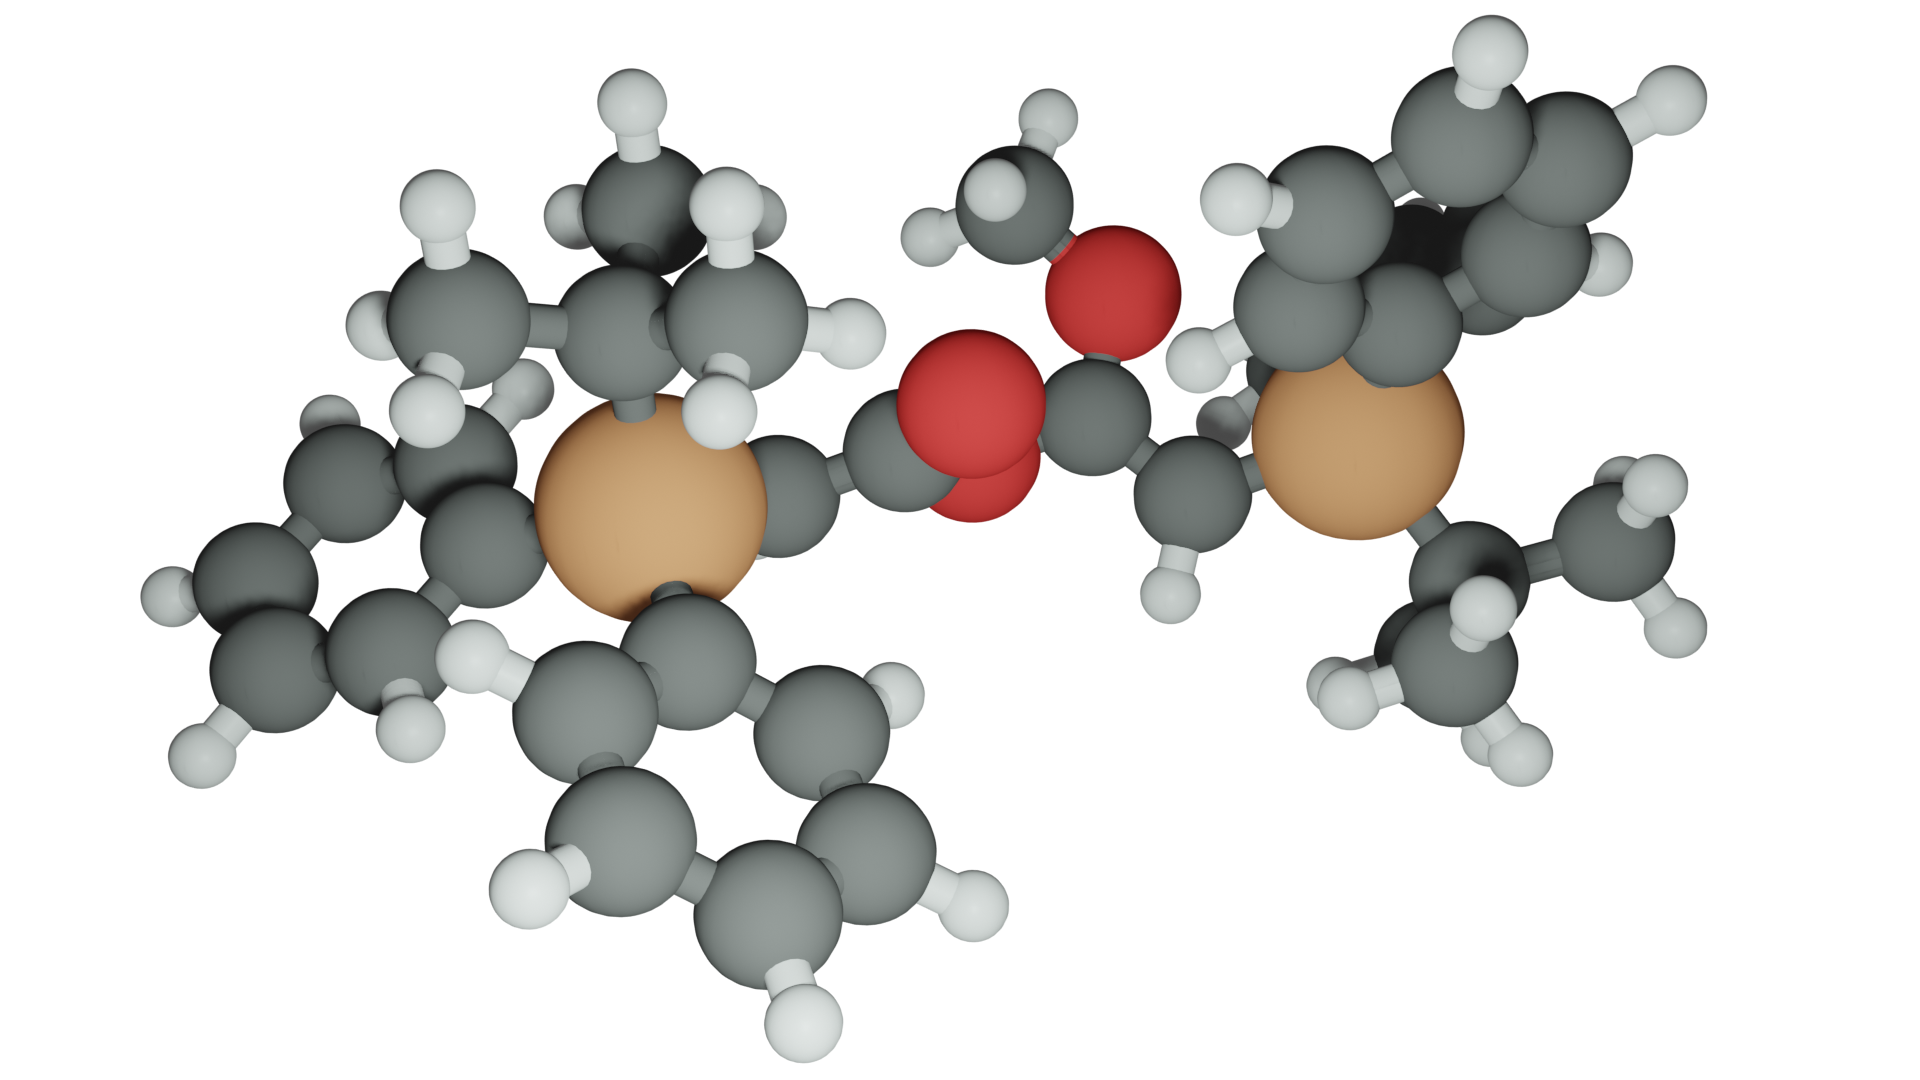
\includegraphics[width=0.3\textwidth]{chapters/project_fragment/images/dimer_render.png}     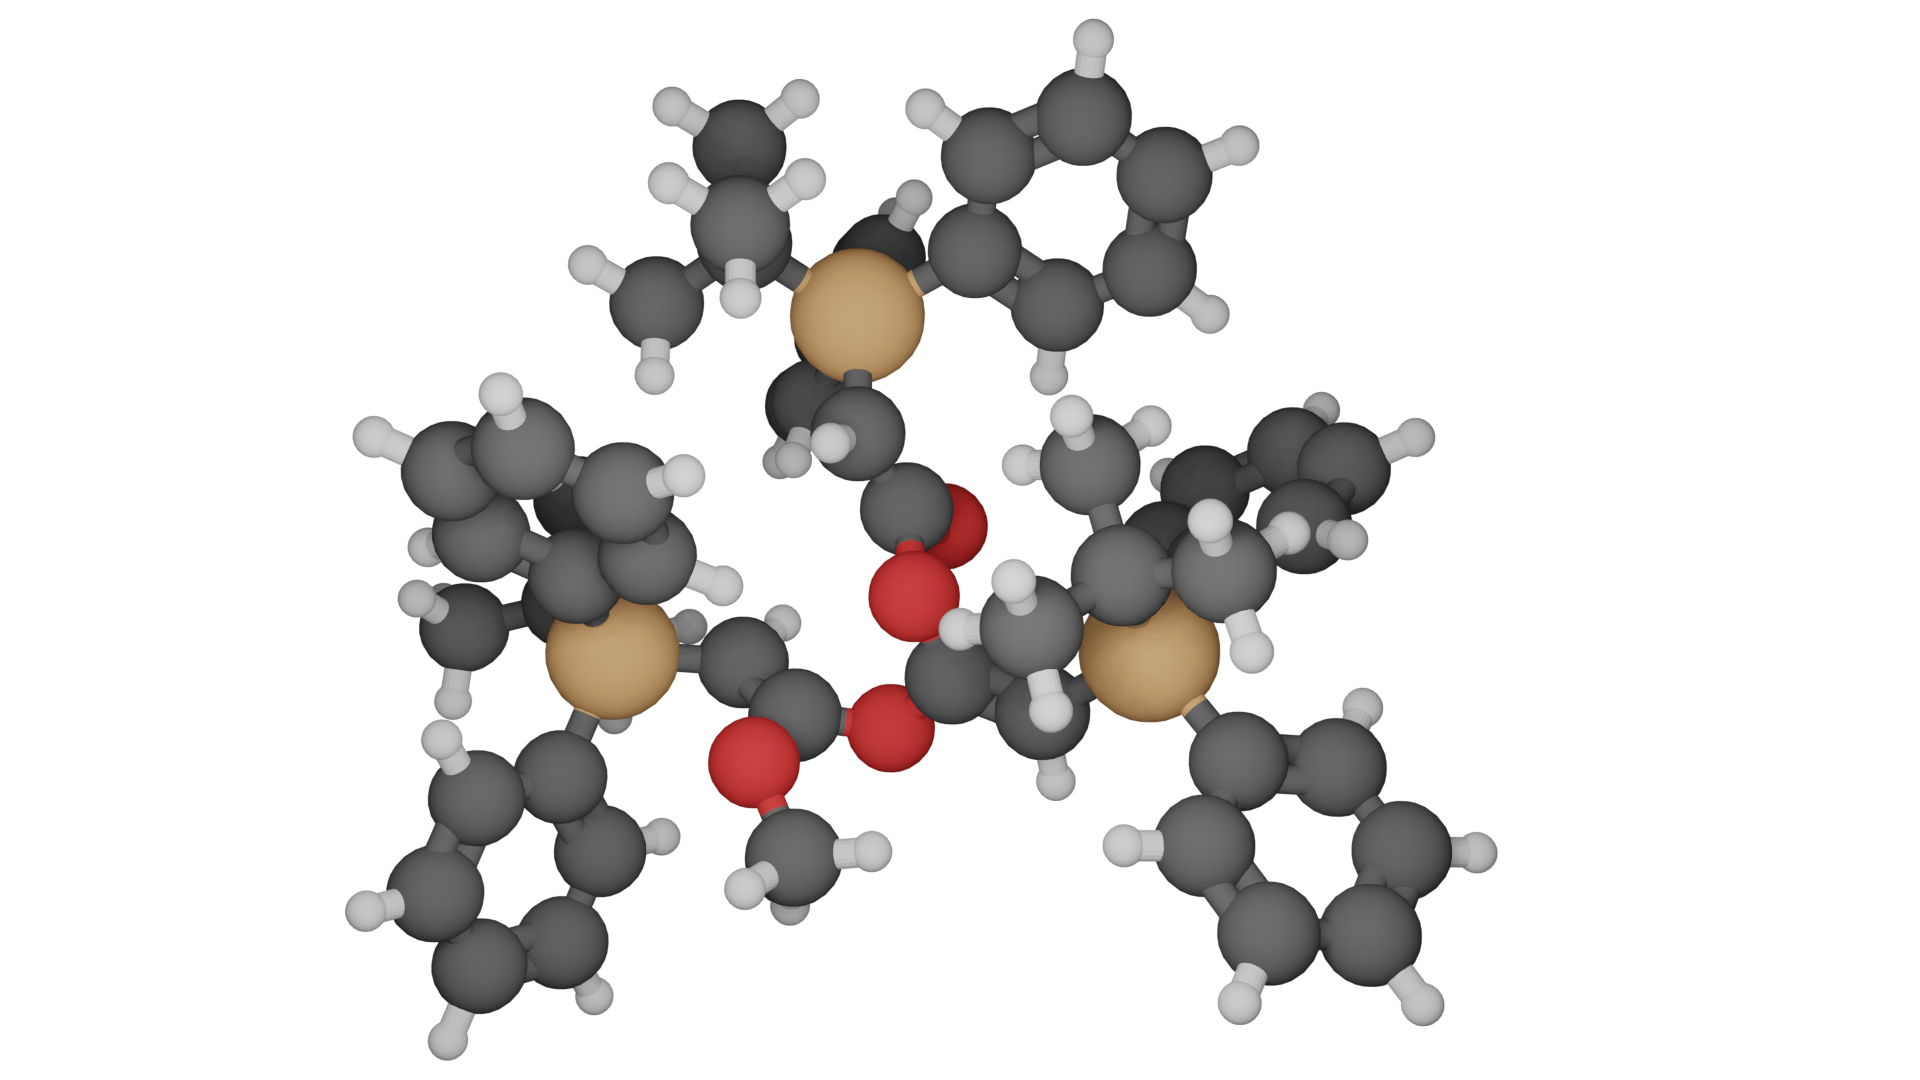
\includegraphics[width=0.3\textwidth]{chapters/project_fragment/images/trimer_render.png}
    \caption[Structures of silyl ketene systems]{Structure of a generic silyl ketene unit (left), the dimer (center) and trimer (right) used for the clustering benchmark.}
    \label{fig:sks}
\end{figure}


% \subsection{Code detail}
% This approach is implemented in the \texttt{AMFC} package, available on \href{https://github.com/amandadumi/molfrag}{Github}.
% The code currently interfaces with Q-Chem 5.0, but can output simple fragment Cartesian coordinate files for easy interfacing with other existing quantum chemistry programs.
% The workflow of the clustering code is described in the list below:
% \begin{enumerate}[itemsep=.02\baselineskip]
%     \item REQUIRED INPUT: Cartesian coordinates, clustering method, descriptor, number of fragments, inter-fragment treatment
%     \item{Determine bonds based on covalent radii}
%     \item if descriptor = MB-scaled
%     \vspace{-0.2\baselineskip}
%         \begin{itemize}[itemsep=.02\baselineskip]
%             \item{Calculate estimate of Mayer bond order}
%         \end{itemize}
%     \vspace{-0.2\baselineskip}
%     else descriptor = Cartesian:
%     \vspace{-0.2\baselineskip}
%     \begin{itemize}[itemsep=.05\baselineskip]
%         \item pass
%     \end{itemize}
%     \vspace{-0.2\baselineskip}
%     \item create fragments based with requested clustering algorithm
%     \item if hydrogen capping is desired, cap fragments
%     \item create input files to calculate fragment at desired inter-fragment treatment
%     \vspace{-0.2\baselineskip}
%     \begin{itemize}[itemsep=.05\baselineskip]
%         \item determine spin state of each fragment. The lowest spin state is enforced for each fragment. Ensure that any radical electrons on one fragment are of opposite spins for neighboring fragments.
%     \end{itemize}
% \end{enumerate}In the oligomer systems, the correct fragmentation is ambiguous and thus correct clustering is not known ahead of time. for these systems the percent error of the fragmented system from supermolecular energy is used as the metric of success.



\section{\label{sec:frag_results} Results and Discussion}

\subsection{Water Clusters}
%In \autoref{subsec:resultswc}, 
% The results of the clustering applied to the water clusters can be seen in Figure~\ref{fig:wc_avg} displayed as the average ARI over the molecular test set. 
The agglomerative, $k$-means, and spectral clustering return the expected clustering as a comparison of the expected and true clustering results with an average ARI of 1 for all descriptors.
This indicates the non-covalently bound water structures are correctly clustered when the number of clusters is predefined.
This is expected as non-covalently bound systems have apparent non-interacting or weakly interacting points are clearly represented by the representation and resolved by the clustering algorithm.
These results suggests these clustering methods could reliably find reasonable fragments for non-covalently bonded systems.

In order to recover the total energy of a water cluster, often more than one water monomer should be included in a fragment, placing importance on clustering methods which allow for the selection of cluster numbers are valuable.
Ideally, the clustering algorithms should resolve to keep individual water molecules intact within each cluster as opposed to separating a molecule between two fragments.\autocite{Herbert2019}
Figure~\ref{fig:descend_cn} demonstrates the fragmentation for spectral clustering with the $G^{xyz}$ descriptor in cases where the number of clusters is lower than the number of water monomers. 
In this case the ideal returned fragments are defined as including one or more water monomers without any segmentation of O-H bonds.
Preservation of covalent bonds is observed for spectral clustering and $k$-means clustering, but not for agglomerative clustering.

 In addition to ensuring preservation of covalent bonds, achieving balanced clusters is also a priority.
The standard deviation of the clusters sizes was used as a metric to probe the clustering method/descriptor pairs.
The \ce{(H2O)_{21}} molecule was partitioned  $N_{frag}=2\dots21$ using the $G^{Mbm}$ and $G^{xyz}$ descriptors with both spectral and $k$-means clustering.
The results shown in Figure~\ref{fig:h2o_variance} demonstrate that spectral clustering with both descriptors return fragments of a similar size over the range tested.  The
$k$-means method with $G^{xyz}$ descriptor  returns fragments of a similar size. Though when paired with the $G^{Mbm}$, requesting a smaller number of fragments returns unevenly sized fragments.

\begin{figure}[h!]
    \centering
    
\includegraphics[width=0.6\textwidth]{chapters/project_fragment/images/descending_cn_simple.png}
   \caption[Visualization of preservation of covalent bonds in \ce{(H2O)_4}]{A demonstrative result for the preservation of covalent bonds in cases when the $N_{frag}$ is less than the $N_{molecules}$. The $N_{frag}$ requested decreases from 4 (requested on the left) to 2 (requesting on the right), clusters are designated by the green outlines. This example is performed with spectral clustering on the Cartesian representation for \ce{(H2O)_4}. Covalent bonds are preserved for all descriptor/clustering algorithm combinations.}
   \label{fig:descend_cn}

\end{figure}
\begin{figure}[h!]
    \centering
    \includegraphics[width=0.6\textwidth]{chapters/project_fragment/images/stddev_lesscluster.eps}
   \caption[Water cluster fragment size standard deviation]{The standard deviation in cluster size for cases when the number of requested clusters is less than the number of monomers. For for \ce{(H2O)_{21}}, the $N_{frag}$ requested increases from 2 to 20. Shown here for the $G^{Mbm}$ and $G^{xyz}$ descriptor.}
   \label{fig:h2o_variance}
\end{figure}

The timing of the clustering itself is another important metric to consider, and the AFMC has negligible cost for generating fragments.
Once the features of the descriptor are calculated, the routine to set up the molecule, generate fragments, and create output files took approximately 2 seconds for all clustering methods on an 4 core laptop with a i5-5200 CPU. 
The AFMC approach thus offers a computationally efficient way to generate fragments which can then be used in combination with any interfragment treatment approaches to estimate the energy and properties of large molecules.


%%%%%%%%%%%%%%%%%%%%%%%%%%%%%%%%%%%%%%%%%%%%%%%%%%%%%%%%%%%%%%%%%%%%%%%%%%%%%%%%%%%%


%%%%%%%%%%%%%%%%%%%%%%%%%%%%%%%%%%%%%%%%%%%%%%%%%%%%%%%%%%%%%%%%%%%%%%%%%%%%%%%%%%%%
\subsection{Methylthiophenes}
% \label{subsec:resultsmt}
\begin{figure}
    \centering
    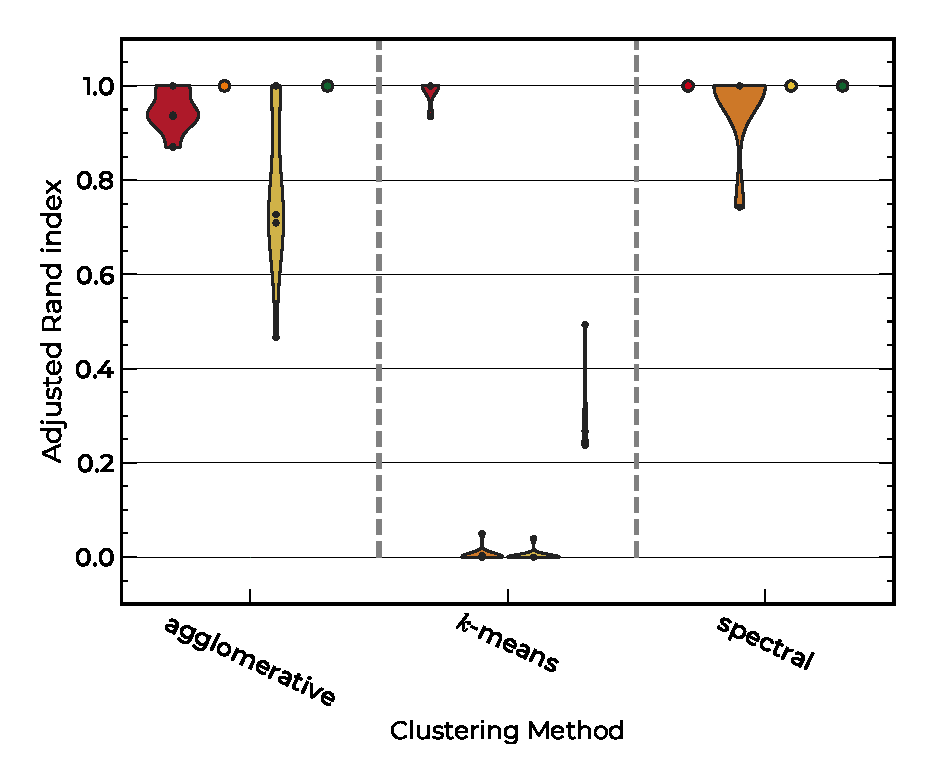
\includegraphics[width=0.45\textwidth]{chapters/project_fragment/images/mt_hf_violin_randidx.eps}
    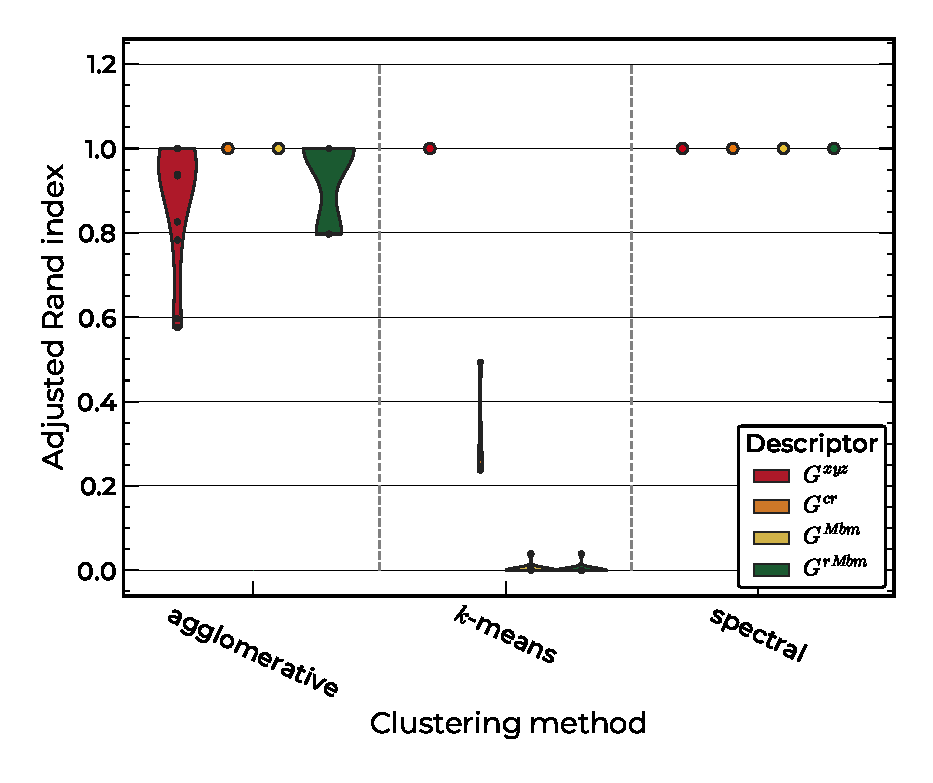
\includegraphics[width=0.45\textwidth]{chapters/project_fragment/images/mt_wb97x-d_violin_randidx.eps}
    \caption[Assessment of UML fragmentation for the methylthiophene test set]{Performance of clustering for the methylthiophene test set, measured as the average ARI across the set of methylthiophenes. The colored dots at 1 indicate successful clustering of the full test set, as the average ARI is 1 for the descriptor/clustering algorithm combination.}
    \label{fig:mt_avg}
\end{figure}


The clustering method performance for the covalently bound methylthiophene tetramers into four fragments are shown in Figure~\ref{fig:mt_avg};
The effects of geometry optimization on the fragmentation results are also presented. 
Optimization are performed at the Hartree-Fock/6-311G** level of theory subfigure a and  $\omega$B97X-D/6-311G** level of theory was used in subfigure b.
Spectral clustering performs well for all molecular representations with no dependence on the descriptor, level of theory, or basis set used. Other clustering methods have a strong dependence on the descriptor used and variation as the level of theory used in the geometry optimization changes. 
These structures are challenging due to the descriptors maintaining less of a block diagonal structure, i.e more non-local interactions.
A less block diagonal structure in the representation means cluster boundaries are much less clear leading to problems for certain unsupervised learning algorithms.
However, as spectral clustering first embeds the representation into a lower dimensional space before clustering, it is able to resolve the primary interactions.
Notably, agglomerative, $k$-means and spectral clustering perform well with the Cartesian descriptor.
% This contrasts with the performance of affinity propagation and the Cartesian descriptor for the water clusters which produced poor fragmentation as indicated by a low average ARI over the test set.
% The aromatic bond length contraction causes the Cartesian descriptor to correctly keep aromatic rings intact, while the non-covalent system broke the system into far too many clusters as described above.
\textcolor{red}{run energy vs speed-up calculations.}
%%%%%%%%%%%%%%%%%%%%%%%%%%%%%%%%%%%%%%%%%%%%%%%%%%%%%%%%%%%%%%%%%%%%%%%%%%%%%%%%%%%%


%%%%%%%%%%%%%%%%%%%%%%%%%%%%%%%%%%%%%%%%%%%%%%%%%%%%%%%%%%%%%%%%%%%%%%%%%%%%%%%%%%%%
\subsection{Silyl Ketene}
\label{subsec:resultssk}

\begin{figure}
    \centering
    \label{fig:sk_trimer_res}
    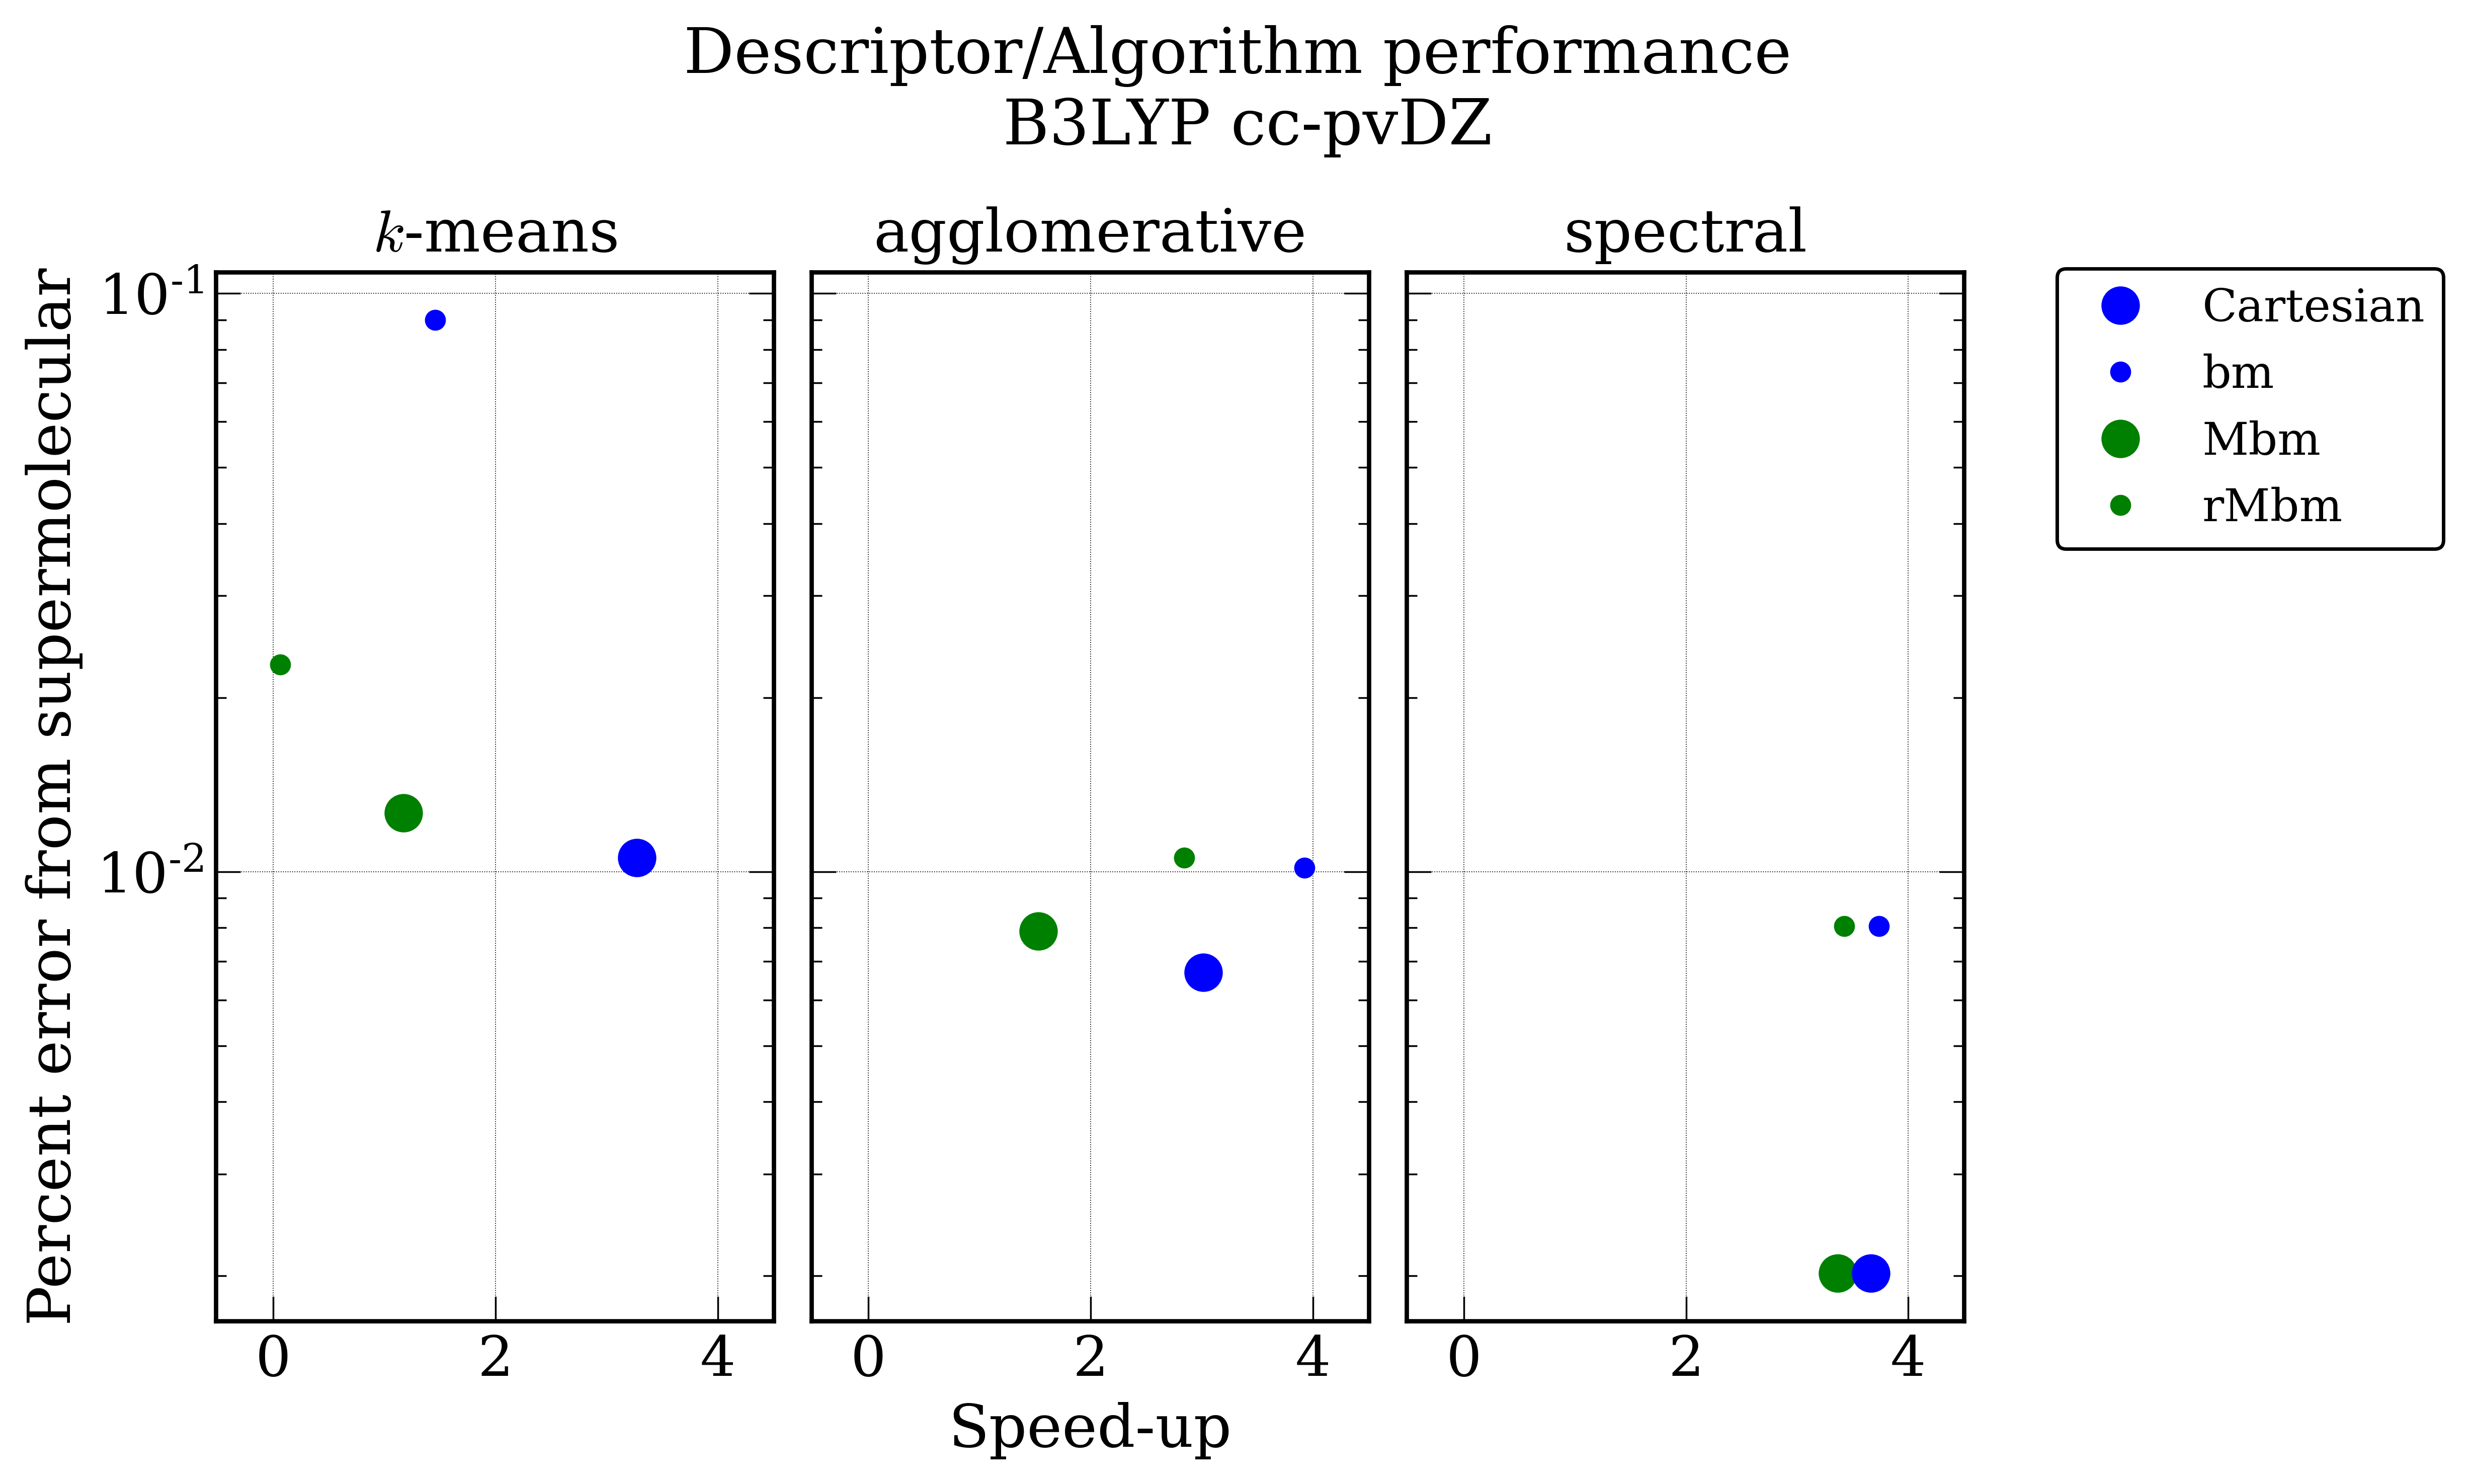
\includegraphics[height=2in]{chapters/project_fragment/images/er_su_trimers_desc_alg.png}
    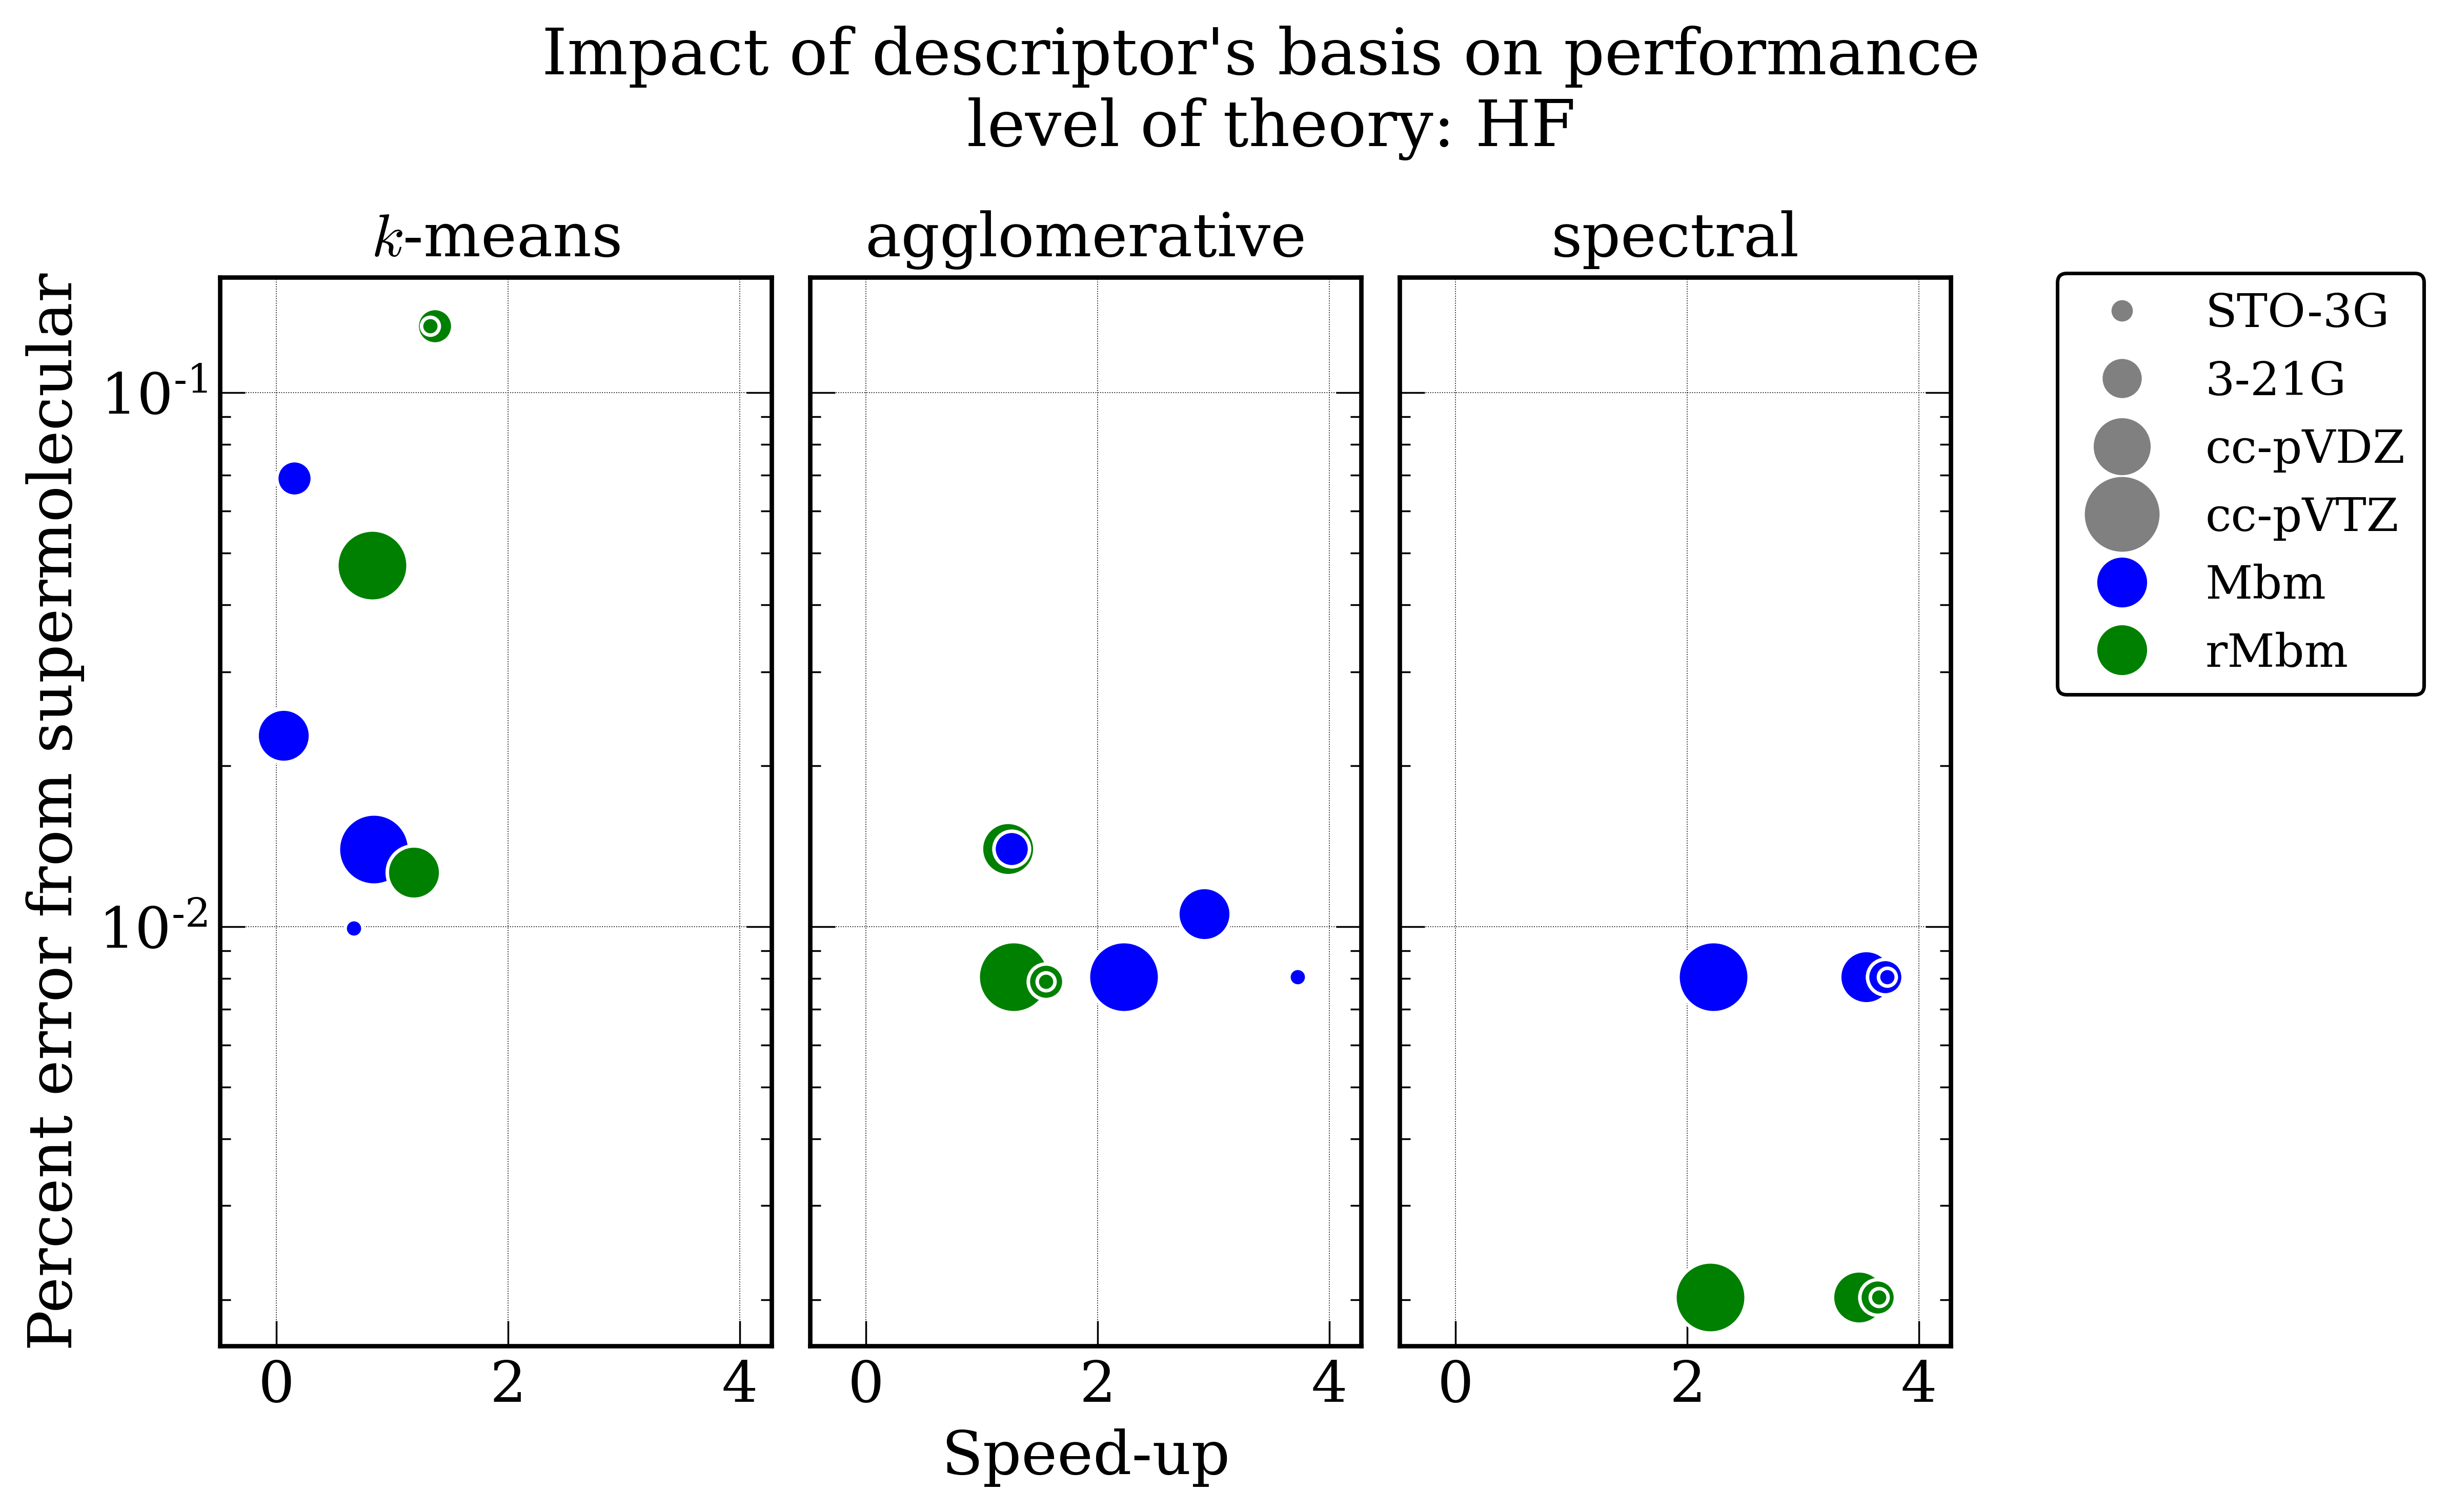
\includegraphics[height=2in]{chapters/project_fragment/images/er_su_trimers_basis.png}
    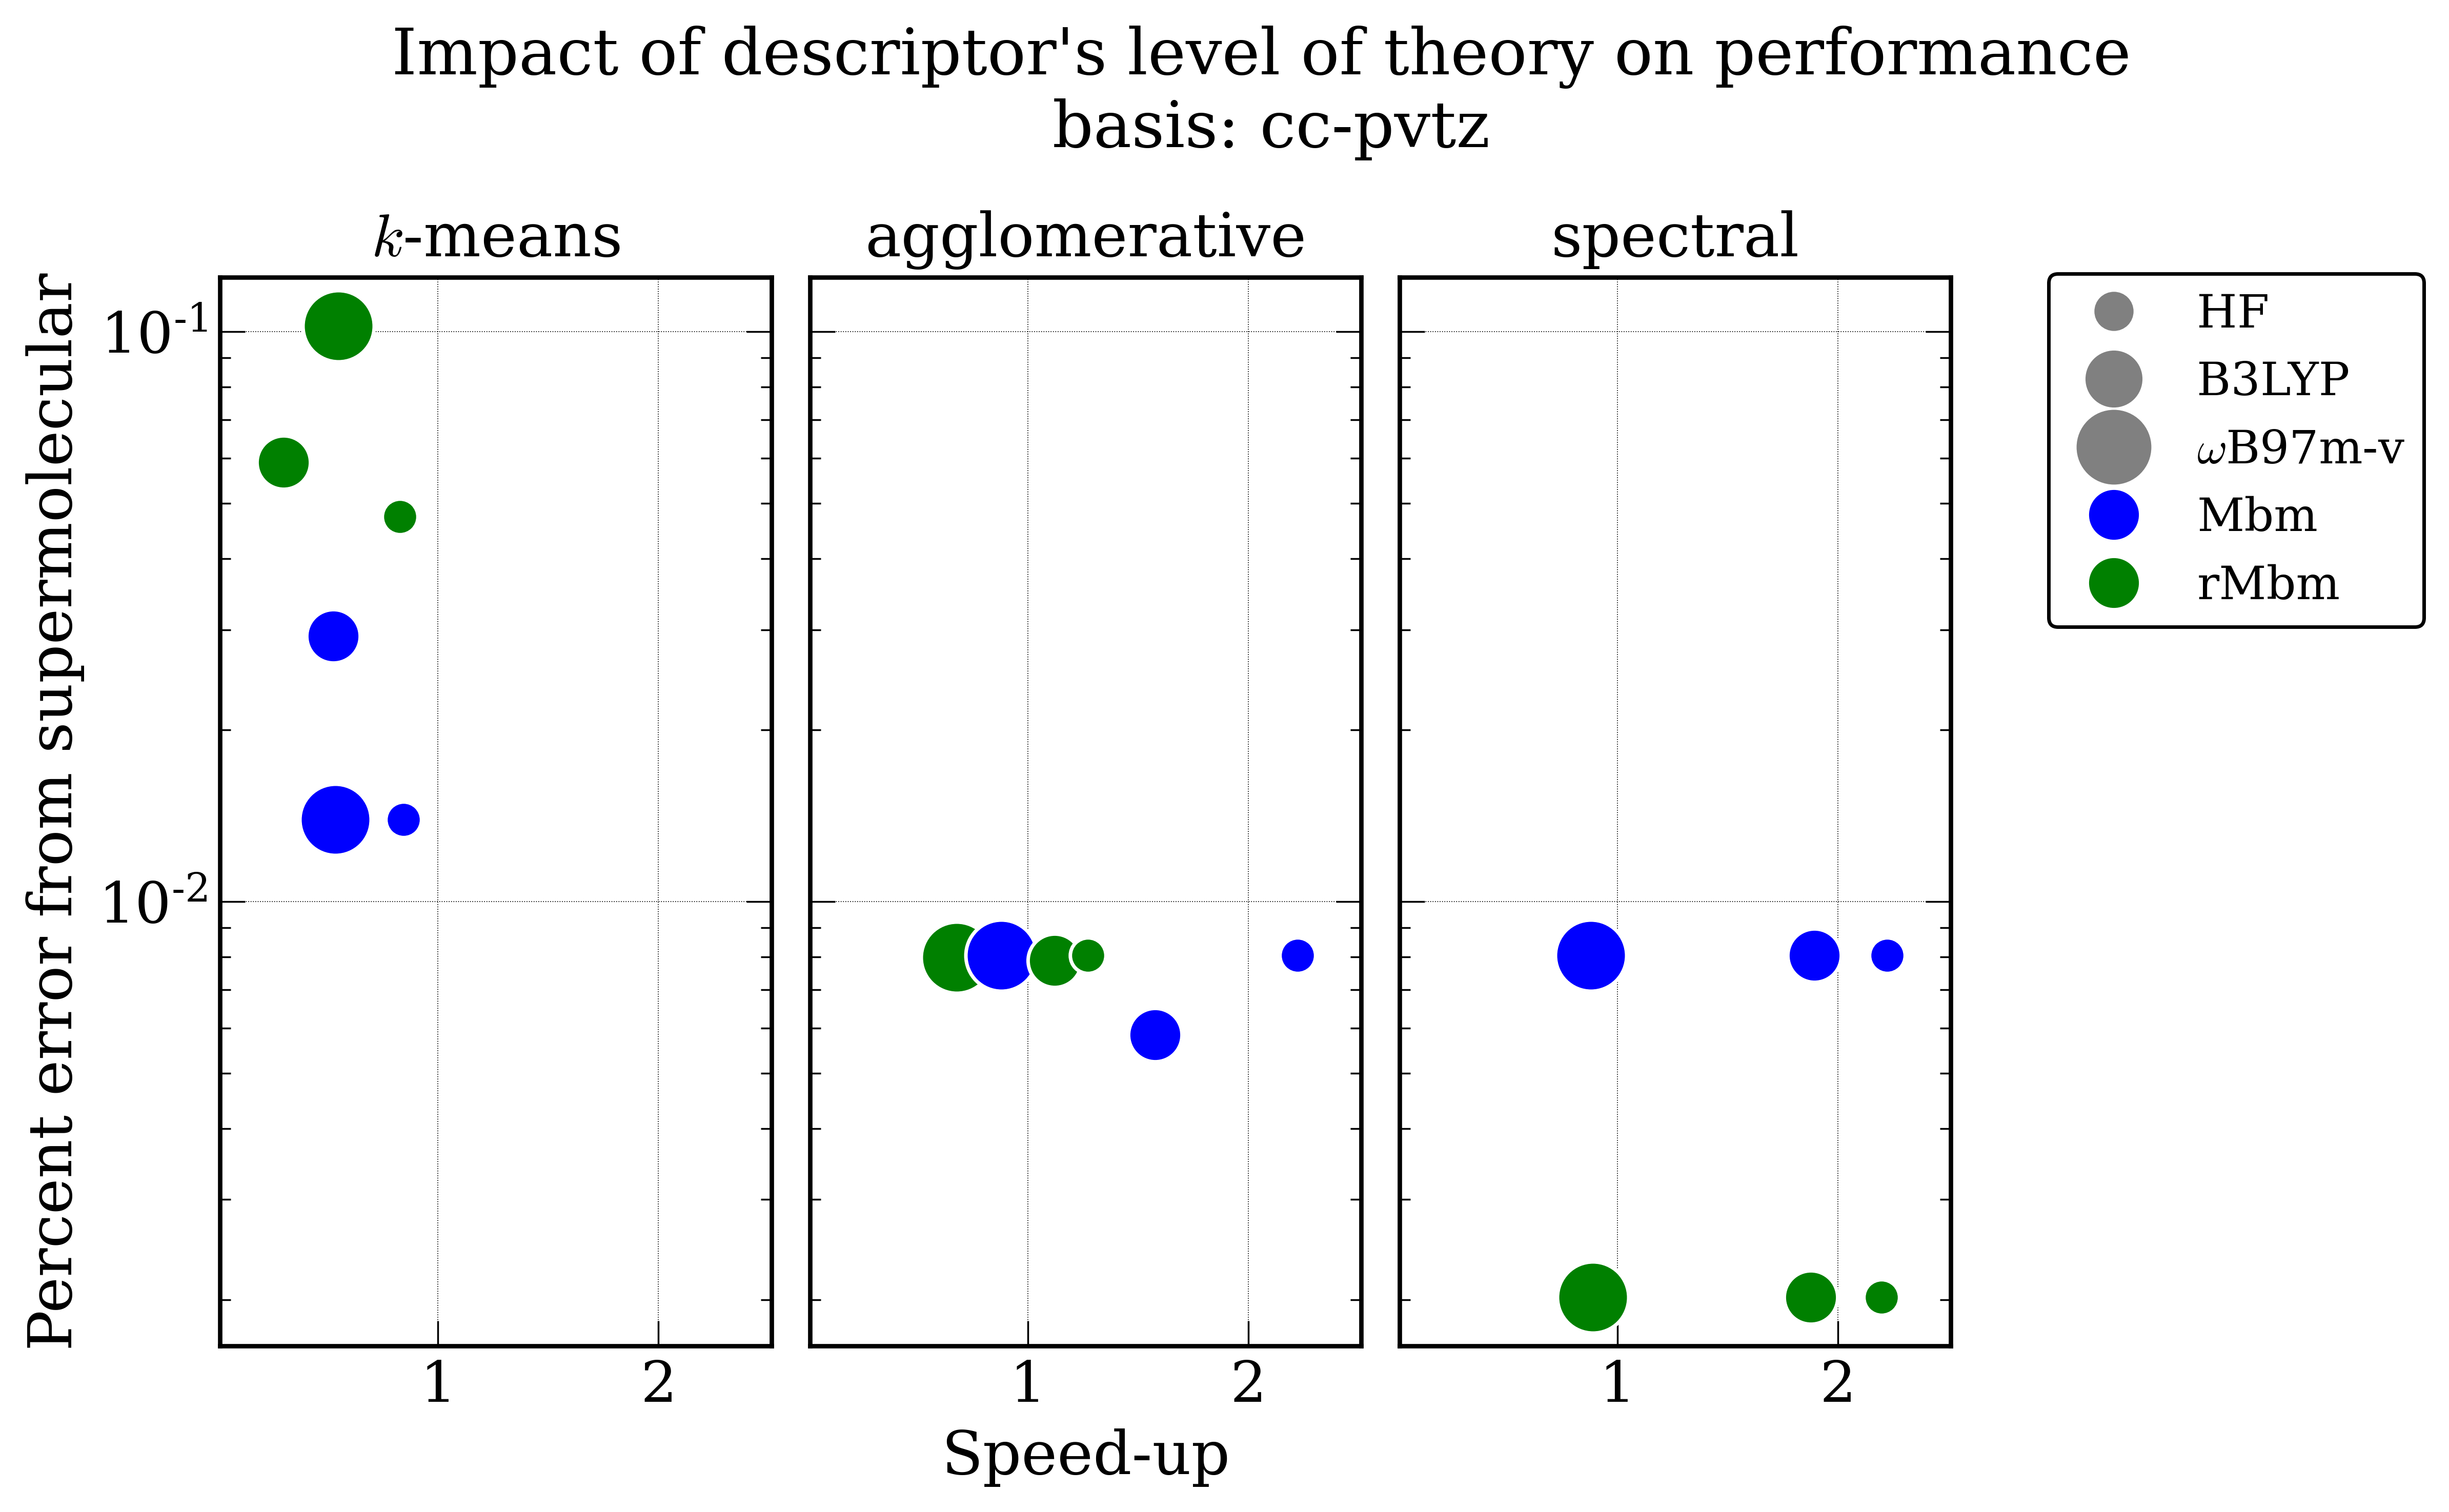
\includegraphics[height=2in]{chapters/project_fragment/images/er_su_trimers_lot.png}

    \caption[Assessment of UML fragmentation schemes on silyl ketene trimers]{Assessment of fragmentation schemes on silyl ketene trimers: Presented is the percent error of the energy and the speedup over the supermolecular calculation for the SK trimer to assess the performance of the fragment approaches and descriptor quality.}
\end{figure}

\begin{figure}
    \centering
    \label{fig:sk_trimer_vis}
        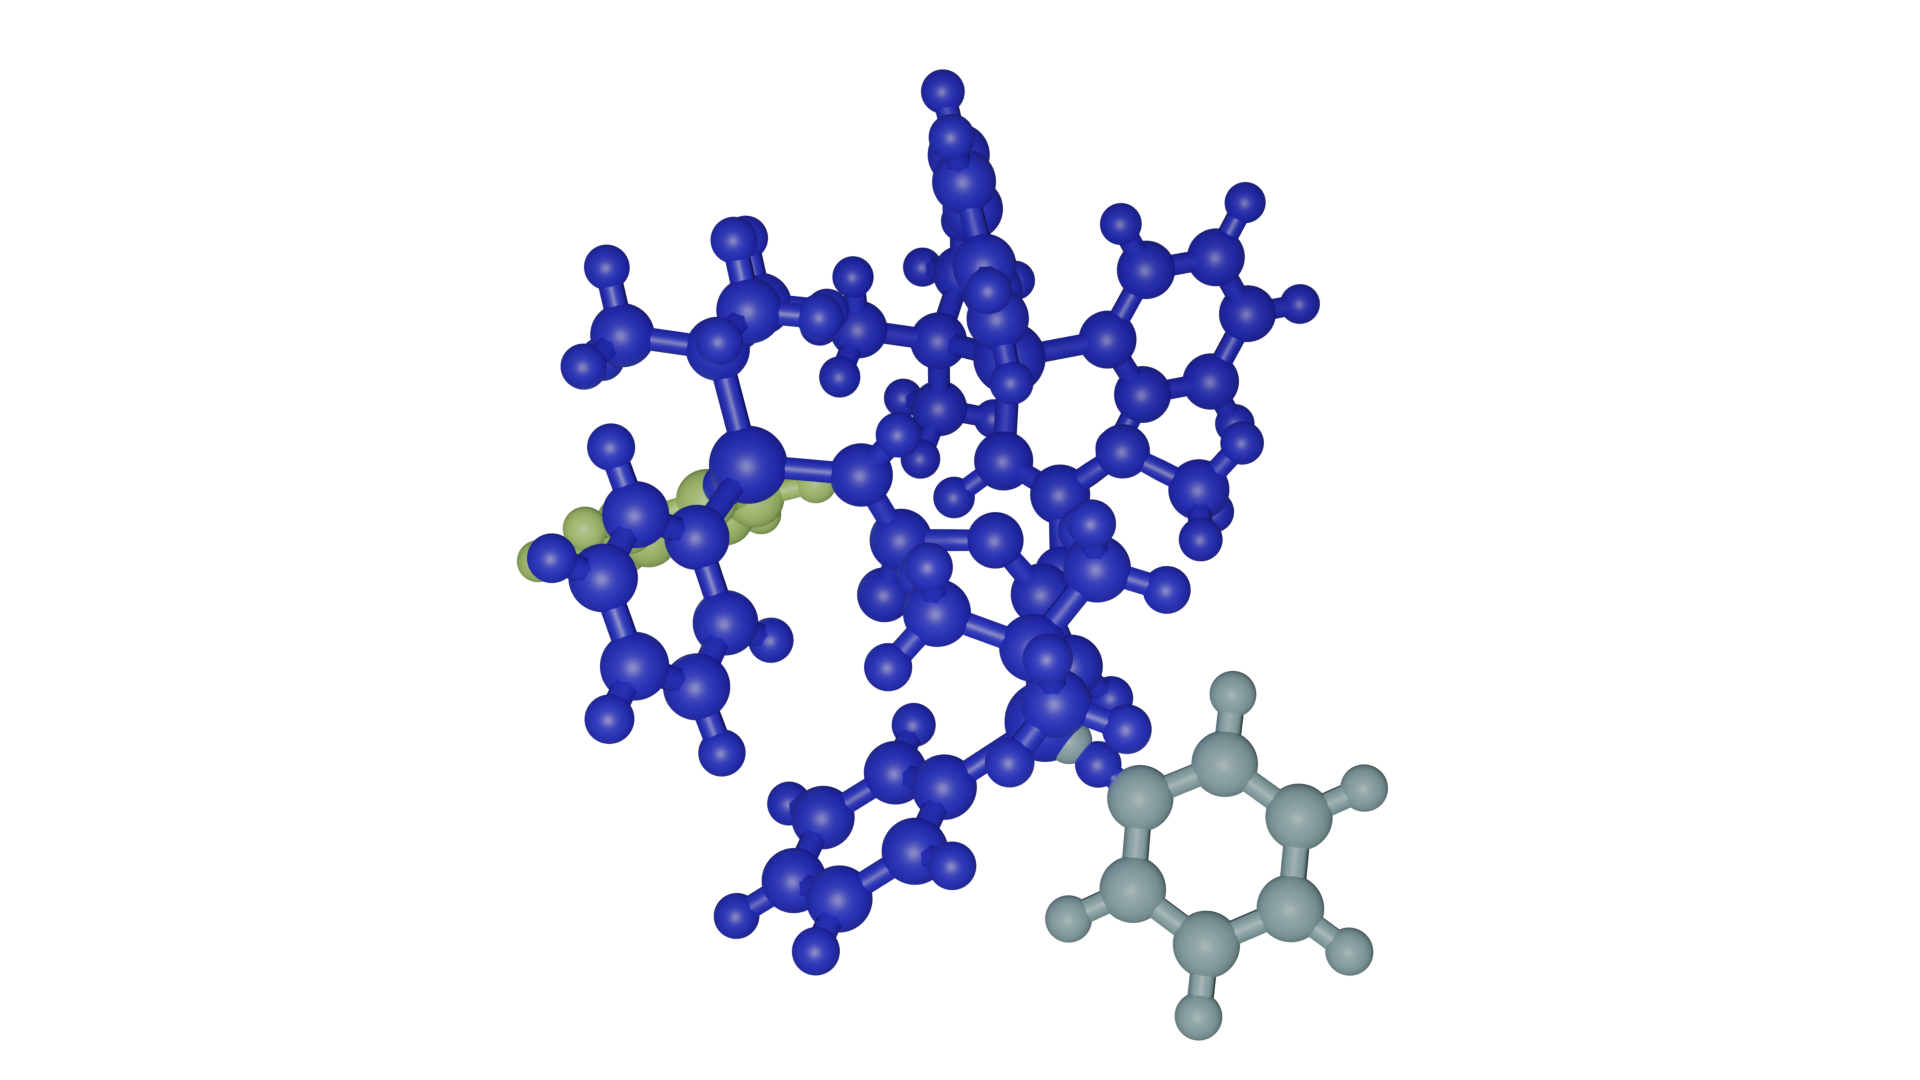
\includegraphics[width=0.4\textwidth]{chapters/project_fragment/images/trimer_a_nrmbm.png}
        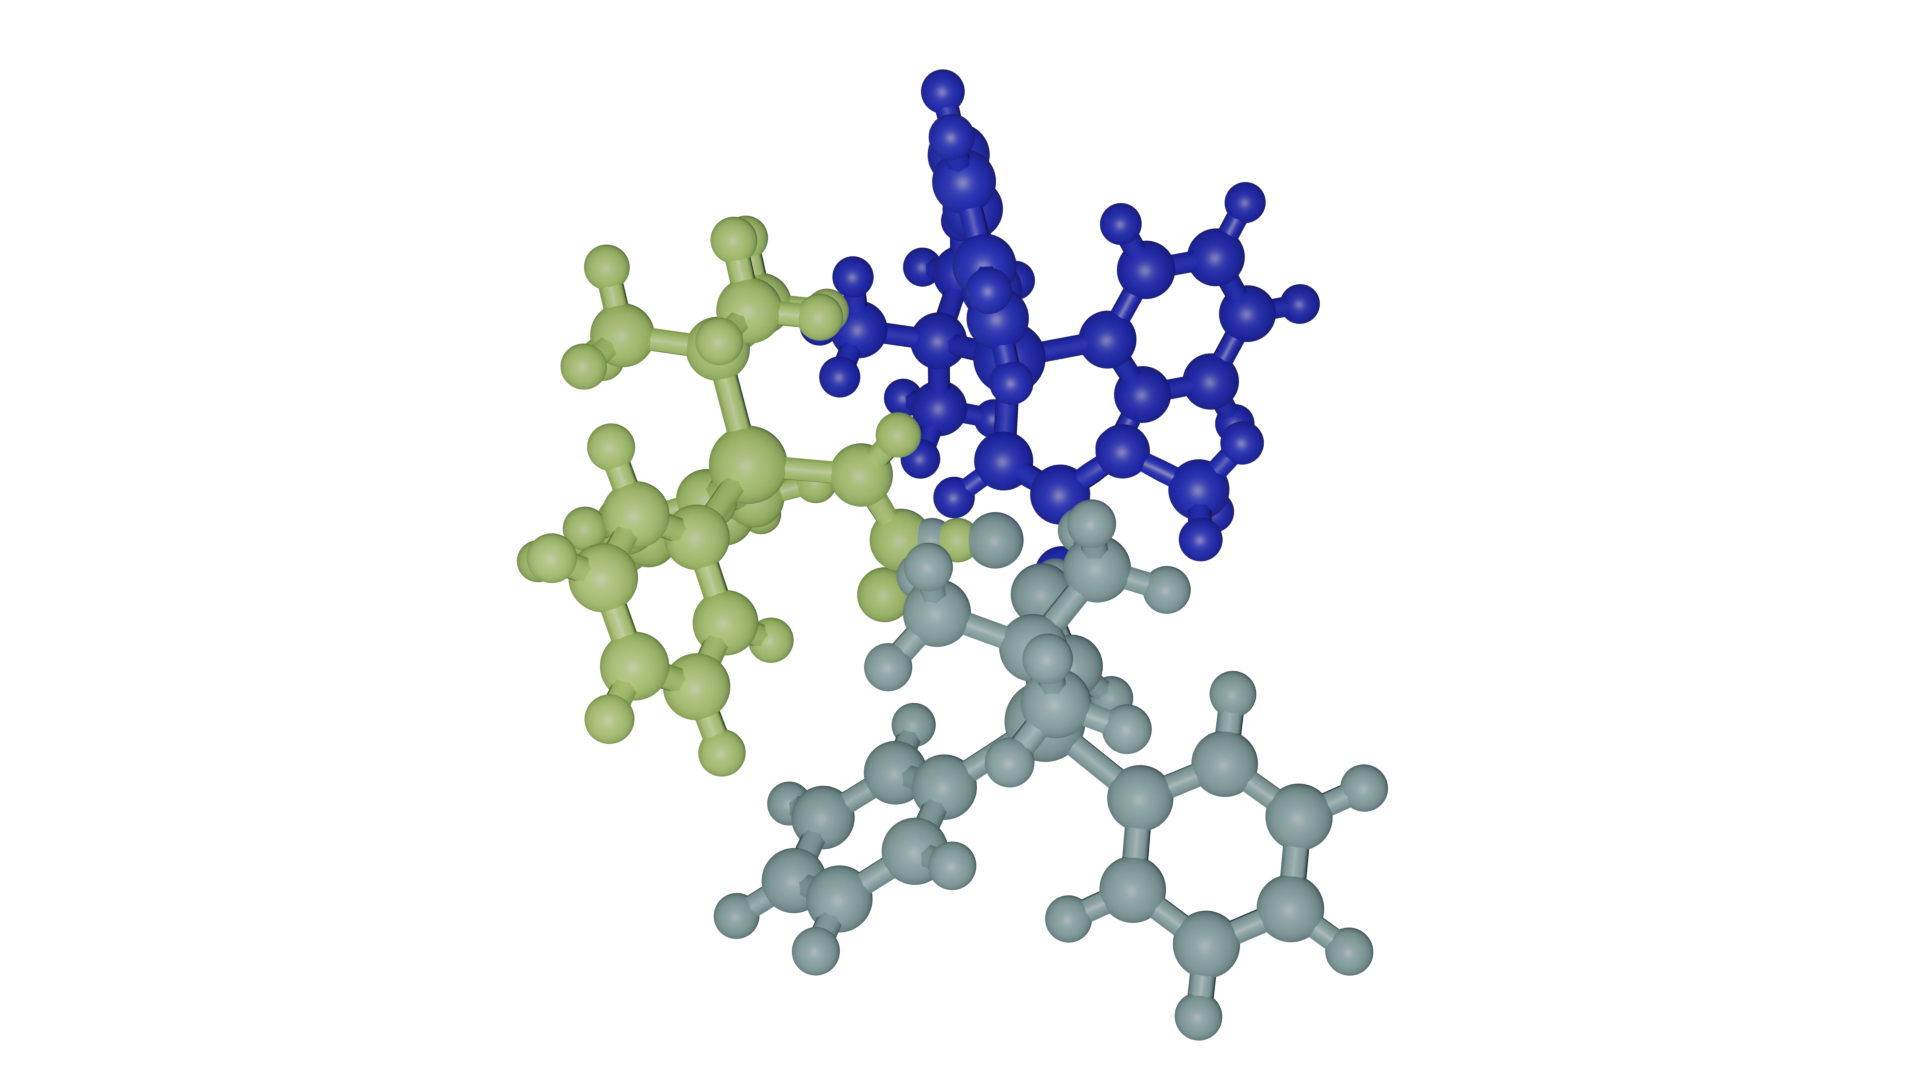
\includegraphics[width=0.4\textwidth]{chapters/project_fragment/images/trimer_s_nrmbm.png}
    \caption[Representative visualization of fragmentation for silyl ketene trimer]{Representative visualization of resulting fragmentation for silyl ketenes. Results from agglomerative (left) and spectral (right) clustering on the $G^{Mbm}$ descriptor. Colors represent fragment identity.}
\end{figure}

Silyl ketenes, realistic systems with more ambiguity in the choice of partitioning, are challenging applications for these clustering approaches.
The dimer results are found in Figure~\ref{fig:sk_dimer_res} and trimer results can be seen in Figure~\ref{fig:sk_trimer_res}.
The findings across the dimers and trimers are comparable and suggest spectral clustering is the most robust clustering algorithm, achieving the lowest errors with the largest speedups across all descriptor/method pairs. 
Interestingly, a fragmentation pattern with the lowest error is found when the covalent radii bond matrix is used for the dimer or the Cartesian descriptor is used for the trimer.
The favorable fragmentation using these purely structure-based descriptors suggests it may be possible to select fragments that result in high accuracies in molecular properties without relying on the incorporation quantum mechanical information in the descriptor for some systems.

Agglomerative clustering produces acceptable fragments, though in general, a larger deviation from the supermolecular result is observed.  
On the other hand, only the Cartesian descriptor with the $k$-means clustering algorithm yields reasonable result, which is likely due to the conserved spatial information allowing for an accurate choice of centroids opposed to representations which employ bonding environment as the features. 
Overall, the clustering approaches investigated are relatively insensitive to the level of theory and basis set used to generate the Mayer bond matrix. which is encouraging as it may allow for future computational savings in future applications on larger more complex systems where a purely structure base descriptor may not incorporate the necessary interaction important to the structure.
If cases arise in larger systems where the quantum mechanics based descriptors become necessary, the low level approximation to the bond order will suffice as long as the bond matrix is meaningful.



\section{Conclusion}
In this work we explore the Automatic Fragmentation of Molecules through Clustering (AFMC) as an automated partitioning scheme for molecular systems.
AFMC approach utilizes UML methods to determine molecular domains in computationally efficient and transferable ways.
Three classes of systems were studied to assess the performance of the AFMC approach: water clusters to investigate non-covalently bonded molecules, methylthiophene tetramers to probe the behavior of AFMC with ring structures, and two silyl ketene oligomers to explore a realistic chemical case with ambiguous fragmentation choices.
Several clustering approaches and molecular representations were tested.
We find that this approach with various clustering methods can accurately identify meaningful molecular domains for non-covalently bound molecular systems (water clusters) and in the case of covalently bonded systems with aromatic units.
Overall, a spectral clustering approach was able to produce balanced and sensible molecular fragments as can be seen by the low error and high speed up for the silyl ketene structures.
The clustering is performed on molecular representations derived from either the molecular structure alone or a low-level quantum mechanics prediction of the Mayer bond matrix.
Both classes of representations performed well for the systems studied, though it is not yet clear whether more intricate, correlation-dependent, bonding schemes will benefit from the quantum mechanical informed descriptors and we aim to explore this in future work. 
The combination of Spectral clustering with the Cartesian descriptor provides the most reliable clustering with minimal preparation cost, thus we recommend this combination for molecules alike to those studied here.
The combination of these descriptors and UML techniques provide a low cost way to determine acceptable fragments for computational chemistry for further, more accurate, quantum mechanical calculations. 



